\documentclass[dvipsnames, aspectratio=169]{beamer}
\usepackage[utf8]{inputenc}
\usepackage{listings}
\usepackage{comment}
\usepackage{soul}
%\usepackage{ulem}
\usepackage{subfig}
\usepackage{pgf-pie}
\setul{}{1pt}
\usepackage[oldenum, olditem]{paralist}
%allow even smaller text
\newcommand\tinytiny{\fontsize{4pt}{3}\selectfont}

\makeatletter
\let\old@lstKV@SwitchCases\lstKV@SwitchCases
\def\lstKV@SwitchCases#1#2#3{}
\makeatother
\usepackage{lstlinebgrd}
\makeatletter
\let\lstKV@SwitchCases\old@lstKV@SwitchCases

\lst@Key{numbers}{none}{%
    \def\lst@PlaceNumber{\lst@linebgrd}%
    \lstKV@SwitchCases{#1}%
    {none:\\%
     left:\def\lst@PlaceNumber{\llap{\normalfont
                \lst@numberstyle{\thelstnumber}\kern\lst@numbersep}\lst@linebgrd}\\%
     right:\def\lst@PlaceNumber{\rlap{\normalfont
                \kern\linewidth \kern\lst@numbersep
                \lst@numberstyle{\thelstnumber}}\lst@linebgrd}%
    }{\PackageError{Listings}{Numbers #1 unknown}\@ehc}}
\makeatother


%disclaimer for Sandia. uncomment and the whole blob goes away @ b80c116300122
\def\sandid{SAND2020-7475 PE}

% \title{Performance Portability with Kokkos}
\title{The Kokkos Lectures}

%BAD misuse of author field
\author{Module 4: Hierarchical Parallelism}

%\author{
%  Jeff Miles \inst{1},
%  Christian Trott \inst{1}
%}
%\institute[shortinst]{\tiny \inst{1} Sandia National Laboratories, \inst{2} Oak Ridge National Laboratory \and \inst{3} Los Alamos National Laboratory}
%\institute[shortinst]{\tiny \inst{1} Sandia National Laboratories}

\usetheme{kokkos}

\newif\ifshort
\newif\ifmedium
\newif\iffull
\newif\ifnotoverview

\newcommand{\TutorialDirectory}{\texttt{Intro-Full}}
\newcommand{\ExerciseDirectory}[1]{\texttt{Exercises/#1/}}
\newcommand{\TutorialClone}{\texttt{Kokkos/kokkos-tutorials/\TutorialDirectory}}

\definecolor{darkgreen}{rgb}{0.0, 0.5, 0.0}
\definecolor{darkred}{rgb}{0.8, 0.0, 0.0}
\definecolor{orange}{rgb}{0.8, 0.33, 0.0}
\definecolor{purple}{rgb}{0.60, 0.20, 0.80}
\colorlet{bodyColor}{blue!20}
\colorlet{patternColor}{orange!30}
\colorlet{policyColor}{green!30}

% http://tex.stackexchange.com/questions/144448/color-a-text-line-in-a-code-lstlisting
\lstnewenvironment{code}[1][]%
{
  %with txfonts: OT1/txr/m/n/10
  %with default fonts: OT1/cmr/m/n/10
  %\fontfamily{cmr}\selectfont
  %\showthe\font
   \noindent
   \minipage{\linewidth}
   %\vspace{0.5\baselineskip}
   \lstset{mathescape, escapeinside={<@}{@>},
moredelim=**[is][{\btHL[fill=patternColor]}]{@pattern}{@pattern},
moredelim=**[is][{\btHL[fill=red!30]}]{@warning}{@warning},
moredelim=**[is][{\btHL[fill=policyColor]}]{@policy}{@policy},
moredelim=**[is][{\btHL[fill=bodyColor]}]{@body}{@body},
moredelim=**[is][{\btHL[fill=red!30]}]{@warning}{@warning},
moredelim=**[is][\color{black}]{@black}{@black},
moredelim=**[is][\color{blue}]{@blue}{@blue},
moredelim=**[is][\bf]{@bold}{@bold},
moredelim=**[is][\it]{@italic}{@italic},
moredelim=**[is][\color{boldblue}\bf]{@boldblue}{@boldblue},
moredelim=**[is][\color{red}]{@red}{@red},
moredelim=**[is][\color{green}]{@green}{@green},
moredelim=**[is][\color{gray}]{@gray}{@gray},
moredelim=**[is][\color{darkgreen}]{@darkgreen}{@darkgreen},
moredelim=**[is][\color{darkred}]{@darkred}{@darkred},
moredelim=**[is][\color{orange}]{@orange}{@orange},
moredelim=**[is][\color{purple}]{@purple}{@purple},
keywords={},
#1}
}
{
  \endminipage
  %\vspace{1.0\baselineskip}
}

\makeatletter
\newif\ifATOlinebackground
\lst@Key{linebackground}{\tiny}{\def\ATOlinebackground{#1}\global\ATOlinebackgroundtrue}
\makeatother

\lstnewenvironment{shell}[1][]{%
  \global\ATOlinebackgroundfalse
  \lstset{language=sh,%
    showstringspaces=false,
    aboveskip=0pt,
    frame=none,
    numbers=none,
    belowskip=2pt,
    breaklines=true,
    #1,
    }
  %\ifATOlinebackground
  \lstset{linebackgroundcolor={
    \ATOlinebackground
  }}
  %\fi
  }{}

\lstnewenvironment{cmake}[1][]{%
  \global\ATOlinebackgroundfalse
  \lstset{language=sh,%
    showstringspaces=false,
    aboveskip=0pt,
    frame=none,
    numbers=none,
    belowskip=2pt,
    breaklines=true,
    #1,
    }
  %\ifATOlinebackground
  \lstset{linebackgroundcolor={
    \ATOlinebackground
  }}
  %\fi
  }{}

\newcommand{\inlinecode}[1]{{\lstset{basicstyle=\ttfamily,keywordstyle={},showstringspaces=false}\lstinline$#1$}}
\newcommand{\inlineshell}[1]{{\lstset{basicstyle=\ttfamily,keywordstyle={},showstringspaces=false}\lstinline$#1$}}

\setbeamercolor{block title}{fg=white, bg=SandiaLightBlue}
\setbeamercolor{block body}{bg=lightgray}
\setbeamercolor{block title alerted}{fg=white, bg=SandiaRed}
\setbeamercolor{block body alerted}{bg=lightgray}



%\usepackage[texcoord,grid,gridunit=mm,gridcolor=red!10,subgridcolor=green!10]{eso-pic}
\usepackage[absolute,overlay]{textpos}





% http://tex.stackexchange.com/questions/8851/how-can-i-highlight-some-lines-from-source-code

\usepackage{pgf, pgffor}
\usepackage{listings}
\usepackage{lstlinebgrd} % see http://www.ctan.org/pkg/lstaddons

\makeatletter
%%%%%%%%%%%%%%%%%%%%%%%%%%%%%%%%%%%%%%%%%%%%%%%%%%%%%%%%%%%%%%%%%%%%%%%%%%%%%%
%
% \btIfInRange{number}{range list}{TRUE}{FALSE}
%
% Test in int number <number> is element of a (comma separated) list of ranges
% (such as: {1,3-5,7,10-12,14}) and processes <TRUE> or <FALSE> respectively

\newcount\bt@rangea
\newcount\bt@rangeb

\newcommand\btIfInRange[2]{%
    \global\let\bt@inrange\@secondoftwo%
    \edef\bt@rangelist{#2}%
    \foreach \range in \bt@rangelist {%
        \afterassignment\bt@getrangeb%
        \bt@rangea=0\range\relax%
        \pgfmathtruncatemacro\result{ ( #1 >= \bt@rangea) && (#1 <= \bt@rangeb) }%
        \ifnum\result=1\relax%
            \breakforeach%
            \global\let\bt@inrange\@firstoftwo%
        \fi%
    }%
    \bt@inrange%
}
\newcommand\bt@getrangeb{%
    \@ifnextchar\relax%
        {\bt@rangeb=\bt@rangea}%
        {\@getrangeb}%
}
\def\@getrangeb-#1\relax{%
    \ifx\relax#1\relax%
        \bt@rangeb=100000%   \maxdimen is too large for pgfmath
    \else%
        \bt@rangeb=#1\relax%
    \fi%
}

%%%%%%%%%%%%%%%%%%%%%%%%%%%%%%%%%%%%%%%%%%%%%%%%%%%%%%%%%%%%%%%%%%%%%%%%%%%%%%
%
% \btLstHL<overlay spec>{range list}
%
% TODO BUG: \btLstHL commands can not yet be accumulated if more than one overlay spec match.
%
\newcommand<>{\btLstHL}[2]{%
  \only#3{\btIfInRange{\value{lstnumber}}{#1}{\color{#2}\def\lst@linebgrdcmd{\color@block}}{\def\lst@linebgrdcmd####1####2####3{}}}%
}%
\makeatother






% http://tex.stackexchange.com/questions/15237/highlight-text-in-code-listing-while-also-keeping-syntax-highlighting
%\usepackage[T1]{fontenc}
%\usepackage{listings,xcolor,beramono}
\usepackage{tikz}

\makeatletter
\newenvironment{btHighlight}[1][]
{\begingroup\tikzset{bt@Highlight@par/.style={#1}}\begin{lrbox}{\@tempboxa}}
{\end{lrbox}\bt@HL@box[bt@Highlight@par]{\@tempboxa}\endgroup}

\newcommand\btHL[1][]{%
  \begin{btHighlight}[#1]\bgroup\aftergroup\bt@HL@endenv%
}
\def\bt@HL@endenv{%
  \end{btHighlight}%
  \egroup
}
\newcommand{\bt@HL@box}[2][]{%
  \tikz[#1]{%
    \pgfpathrectangle{\pgfpoint{1pt}{0pt}}{\pgfpoint{\wd #2}{\ht #2}}%
    \pgfusepath{use as bounding box}%
    \node[anchor=base west, fill=orange!30,outer sep=0pt,inner xsep=1pt, inner ysep=0pt, rounded corners=3pt, minimum height=\ht\strutbox+1pt,#1]{\raisebox{1pt}{\strut}\strut\usebox{#2}};
  }%
}
\makeatother



\usetikzlibrary{calc}
\usepackage{xparse}%  For \NewDocumentCommand

% tikzmark command, for shading over items
\newcommand{\tikzmark}[1]{\tikz[overlay,remember picture] \node (#1) {};}

\makeatletter
\NewDocumentCommand{\DrawBox}{s O{}}{%
    \tikz[overlay,remember picture]{
    \IfBooleanTF{#1}{%
        \coordinate (RightPoint) at ($(left |- right)+(\linewidth-\labelsep-\labelwidth,0.0)$);
    }{%
        \coordinate (RightPoint) at (right.east);
    }%
    \draw[red,#2]
      ($(left)+(-0.2em,0.9em)$) rectangle
      ($(RightPoint)+(0.2em,-0.3em)$);}
}

\NewDocumentCommand{\DrawBoxWide}{s O{}}{%
    \tikz[overlay,remember picture]{
    \IfBooleanTF{#1}{%
        \coordinate (RightPoint) at ($(left |- right)+(\linewidth-\labelsep-\labelwidth,0.0)$);
    }{%
        \coordinate (RightPoint) at (right.east);
    }%
    \draw[red,#2]
      ($(left)+(-\labelwidth,0.9em)$) rectangle
      ($(RightPoint)+(0.2em,-0.3em)$);}
}

\NewDocumentCommand{\DrawBoxWideBlack}{s O{}}{%
    \tikz[overlay,remember picture]{
    \IfBooleanTF{#1}{%
        \coordinate (RightPoint) at ($(left |- right)+(\linewidth-\labelsep-\labelwidth,0.0)$);
    }{%
        \coordinate (RightPoint) at (right.east);
    }%
    \draw[black,#2]
      ($(left)+(-\labelwidth,0.9em)$) rectangle
      ($(RightPoint)+(0.2em,-0.3em)$);}
}
\makeatother

\usetikzlibrary{positioning}

\usetikzlibrary{shapes}

\hypersetup{
    colorlinks=true,
    linkcolor=blue,
    filecolor=magenta,
    urlcolor=cyan,
}



\shortfalse
\mediumtrue
\fulltrue
\notoverviewtrue

\begin{document}

% \begin{frame}
%   \titlepage
% \end{frame}
% 
%==============================================================================

\begin{frame}{NVIDIA's NVLABS LOGISTICS (1)}

\textbf{\large SOFTWARE FOR LAB}

\vspace{10pt}

\textbf{Remote Desktop Software:} \\
\begin{itemize}
\item {Download NoMachine now for best performance from \\
 \textbf{\ul{www.nomachine.com/download}}}
\item {Alternatively you may use a VNC client or the provided browser-based VNC option}
\end{itemize}

\vspace{10pt}

\textbf{SSH Access Software (optional):}
\begin{itemize}
\item PuTTy for Windows can be downloaded from \textbf{\ul{www.putty.org}}
\item{Alternatively you may use a provided browser-based SSH option}
\end{itemize}

\end{frame}

%==============================================================================

\begin{frame}{NVIDIA's NVLABS LOGISTICS (2)}

\textbf{\Large CONNECTION INSTRUCTIONS}
\begin{itemize}
\item {Navigate to \textbf{\ul{nvlabs.qwiklab.com}}}
\item {Login or create a new account}
\item {Select the \textbf{Instructor-Led Hands-on Labs} Class}
\item {Find the lab called \textbf{Kokkos, ...}, select it, click Select, and finally click Start}
\item {After a short wait, lab instance Connection information will be shown}
\item {Please ask Lab Assistants for help!}
\end{itemize}

\end{frame}

%==============================================================================



\begin{frame}
	\titlepage
\end{frame}

\begin{frame}[fragile]{Welcome to Kokkos}

\textbf{Online Resources}:

\begin{itemize}
        \item \url{https://github.com/kokkos}:
                \begin{itemize}
                        \item Primary Kokkos GitHub Organization
                \end{itemize}
        \item \url{https://kokkos.org/kokkos-core-wiki/videolectures.html}
                \begin{itemize}
			\item{Slides, recording and Q\&A for the Lectures}
                \end{itemize}
        \item \url{https://kokkos.org/kokkos-core-wiki}:
                \begin{itemize}
                        \item Programming guide and API reference documentation
                \end{itemize}
        \item \url{https://kokkosteam.slack.com}:
                \begin{itemize}
                        \item Slack channel for Kokkos.
                        \item Please join: fastest way to get your questions answered.
                        \item Can whitelist domains, or invite individual people.
                \end{itemize}
\end{itemize}

\end{frame}


\begin{frame}[fragile]{Lecture Series Outline}

\begin{itemize}
        \item 07/17 Module 1: Introduction, Building and Parallel Dispatch
        \item 07/24 Module 2: Views and Spaces
        \item 07/31 Module 3: Data Structures + MultiDimensional Loops
        \item \textbf{08/07 Module 4: Hierarchical Parallelism}
        \item 08/14 Module 5: Tasking, Streams and SIMD
        \item 08/21 Module 6: Internode: MPI and PGAS
        \item 08/28 Module 7: Tools: Profiling, Tuning and Debugging
        \item 09/04 Module 8: Kernels: Sparse and Dense Linear Algebra
        \item 09/11 Reserve Day
\end{itemize}

\end{frame}

\begin{frame}[fragile]{Module 3: Summary}

	\textbf{MDRangePolicy}
        \begin{itemize}
                \item Tightly nested loops (similar to OpenMP collapse clause)
                \item Available with \texttt{parallel\_for} and \texttt{parallel\_reduce}
                \item Tiling strategy over the iteration space
                \item Control iteration pattern at compile time
        \end{itemize}

\begin{code}[keywords={double,Iterate,Left,Right,int,MDRangePolicy,Rank}]
View<double**,LayoutLeft> A("A",N0,N1);
parallel_for("Label",
  MDRangePolicy<Rank<2,Iterate::Left,Iterate::Left>>(
	{0,0},{N0,N1}),
  KOKKOS_LAMBDA(int i, int j) {
    A(i,j) = 1000.0 * i + 1.0*j;
});
\end{code}

\end{frame}

\begin{frame}[fragile]{Module 3: Summary}

	\textbf{Subviews}
        \begin{itemize}
                \item Taking slices of Views
                \item Similar capability as provided by Matlab, Fortran, or Python
                \item {Prefer the use of \texttt{auto} for the type
\begin{code}[keywords={View,int,subview,ALL,make_pair}]
View<int ***> v("v", N0, N1, N2);
auto sv = subview(v, i0, ALL, make_pair(start,end));
\end{code}}
        \end{itemize}

        \vspace{10pt}
        \textbf{Unmanaged Views}
        \begin{itemize}
                \item Interoperability with externally allocated arrays
                \item No reference counting, memory not deallocated at destruction
                \item { User is responsible for insuring proper dynamic and/or static extents, MemorySpace, Layout, etc.
\begin{code}[keywords={View, float, LayoutRight, HostSpace, MemoryTraits, Unmanaged}]
View<float**, LayoutRight, HostSpace>
  v_unmanaged(raw_ptr, N0, N1);
\end{code}}
        \end{itemize}

\end{frame}

\begin{frame}[fragile]{Module 3: Summary}

	\textbf{Atomic operations}
        \begin{itemize}
                \item Atomic functions available on the host or the device (e.g. \texttt{Kokkos::atomic\_add})
                \item {Use \texttt{Atomic} memory trait for atomic accesses on Views
\begin{code}[keywords={View,int,MemoryTraits,Atomic}]
View<int*> v("v", N0);
View<int*, MemoryTraits<Atomic>> v_atomic = v;
\end{code}}
                \item Use \texttt{ScatterView} for scatter-add parallel pattern
        \end{itemize}

        \vspace{10pt}
	\textbf{Dual Views}
        \begin{itemize}
                \item For managing data synchronization between host and device
 		\item Helps in codes with no holistic view of data flow
		\begin{itemize}
                   \item In particular when porting codes incrementally
                \end{itemize}
        \end{itemize}

\end{frame}
\begin{frame}{Module 4: Hierarchical Parallelism (08/07)}

	\vspace{5pt}
	\textbf{Hierarchical Parallelism}
	\begin{itemize}
        \item How to leverage more parallelism through nested loops.
        \item The concept of Thread-Teams and Vectorlength.
	\end{itemize}

	\vspace{5pt}
	\textbf{Scratch Space}
	\begin{itemize}
        \item Getting temporary workspace in kernels.
        \item Leveraging GPU Shared Memory.
	\end{itemize}

        \vspace{5pt}
        \textbf{Unique Token}
        \begin{itemize}
        \item How to acquire safely per-thread resources.
        \end{itemize}

\end{frame}

\begin{comment}
try a scan and fill for fill array?
\end{comment}

%==========================================================================

\begin{frame}[fragile]

  {\Huge Hierarchical parallelism}

  \vspace{10pt}

  {\large Finding and exploiting more parallelism in your computations.}

  \vspace{20pt}

  \textbf{Learning objectives:}
  \begin{itemize}
    \item {Similarities and differences between outer and inner levels of parallelism}
    \item {Thread teams (league of teams of threads)}
    \item {Performance improvement with well-coordinated teams}
  \end{itemize}

  \vspace{-20pt}

\end{frame}

%==========================================================================

\begin{frame}[fragile]{Example: inner product (0)}

  \ul{\textbf{(Flat parallel) Kernel:}}

  \vspace{-3pt}

  \begin{code}[keywords={}]
Kokkos::parallel_reduce("yAx",N,
  KOKKOS_LAMBDA (const int row, double & valueToUpdate) {
    double thisRowsSum = 0;
    for (int col = 0; col < M; ++col) {
      thisRowsSum += @blueA@blue(row,col) * @darkgreenx@darkgreen(col);
    }
    valueToUpdate += @darkredy@darkred(row) * thisRowsSum;
  }, @orangeresult@orange);
  \end{code}

 \begin{tikzpicture}[remember picture, overlay]
    \node [shift={(-8.0cm,1.10cm)}]  at (current page.south east)
      {%
      \begin{tikzpicture}[remember picture, overlay]
        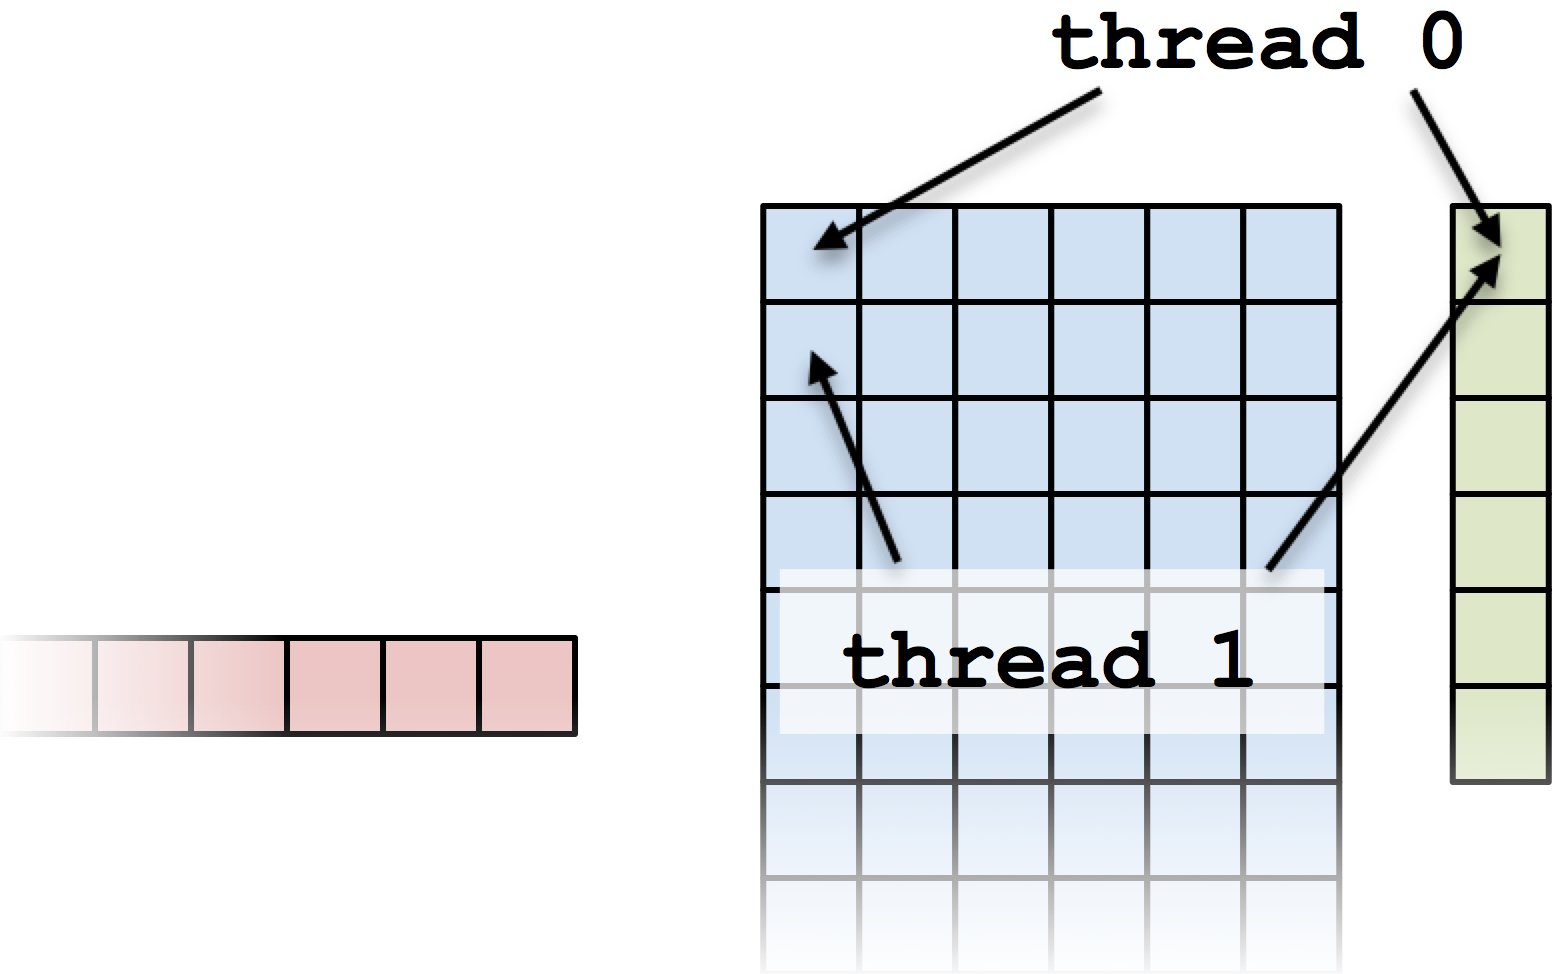
\includegraphics[width=0.60\textwidth]{figures/InnerProductExample_Flat}
      \end{tikzpicture}
      };
  \end{tikzpicture}

  \vspace{10pt}
  \pause

  \begin{columns}[t,onlytextwidth]
    \column{.60\textwidth}
    \textbf{Problem:} What if we don't have enough rows to saturate the GPU?
    \column{.40\textwidth}
  \end{columns}

  \vspace{10pt}
  \pause

  \textbf{Solutions?}
  \pause
  \vspace{-5pt}

  \begin{itemize}
    \item{Atomics}
    \item{Thread teams}
  \end{itemize}

\end{frame}

%==========================================================================
\iffull
\begin{frame}[fragile]{Example: inner product (1)}

  \ul{\textbf{Atomics kernel:}}

  \vspace{-3pt}

  \begin{code}[keywords={}]
Kokkos::parallel_for("yAx", N*M,
  KOKKOS_LAMBDA (const size_t index) {
    const int row = extractRow(index);
    const int col = extractCol(index);
    atomic_add(&@orangeresult@orange, @redy@red(row) * @blueA@blue(row,col) * @darkgreenx@darkgreen(col));
  });
  \end{code}

 \begin{tikzpicture}[remember picture, overlay]
    \node [shift={(-8.0cm,1.10cm)}]  at (current page.south east)
      {%
      \begin{tikzpicture}[remember picture, overlay]
        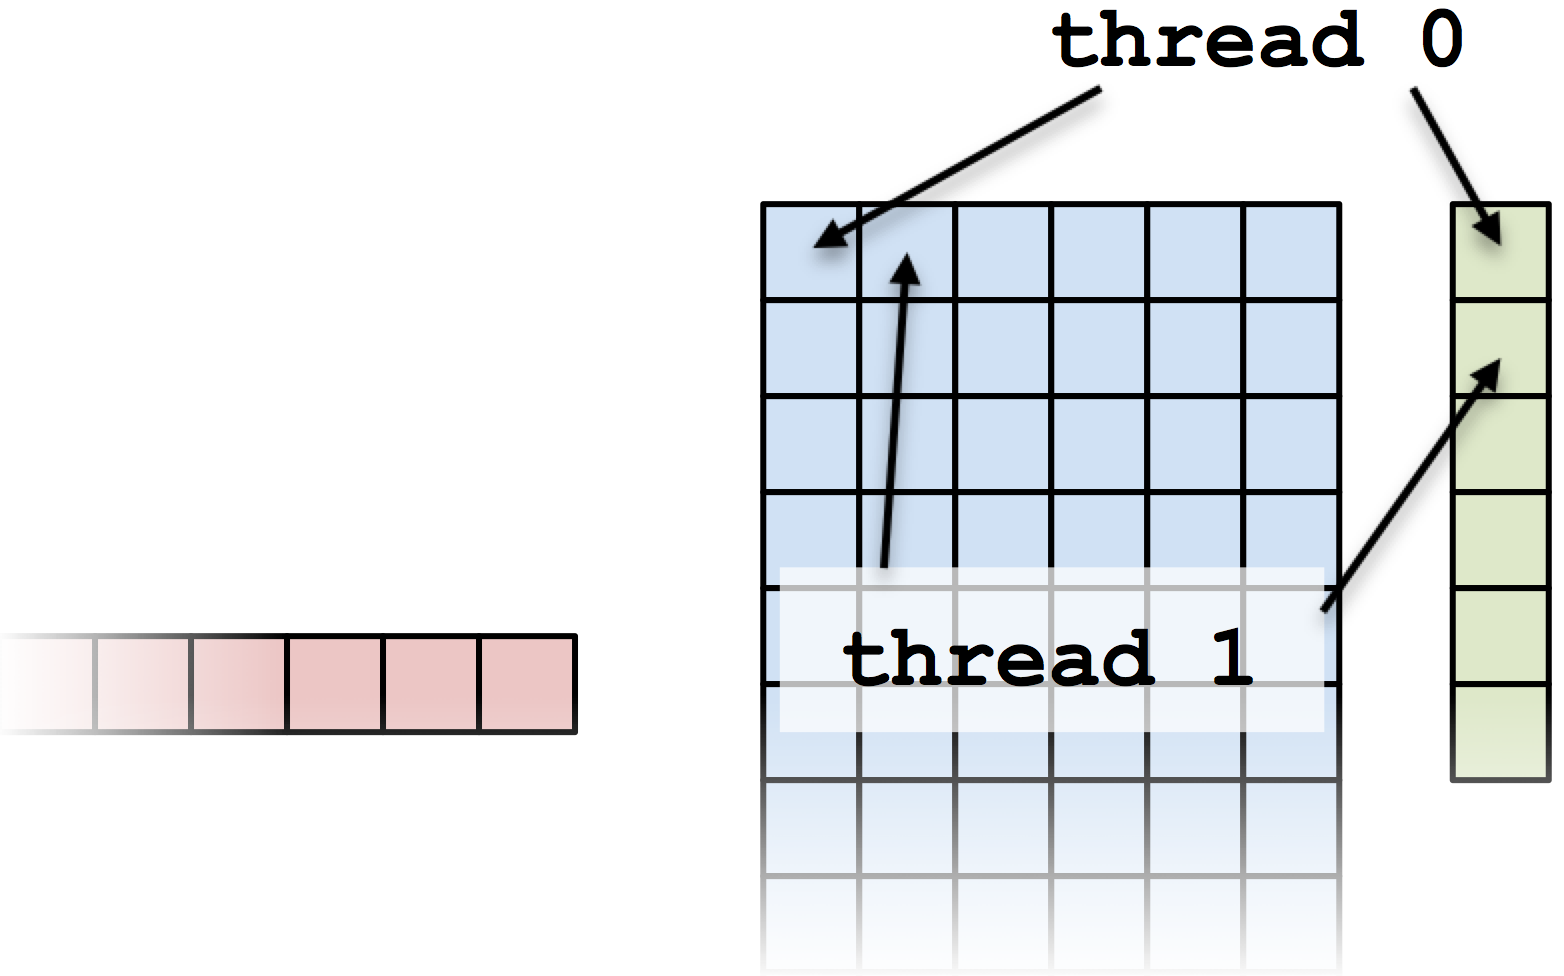
\includegraphics[width=0.60\textwidth]{figures/InnerProductExample_Atomics}
      \end{tikzpicture}
      };
  \end{tikzpicture}

  \vspace{10pt}
  \pause

  \begin{columns}[t,onlytextwidth]
    \column{.60\textwidth}
    {\color{red}\textbf{Problem:}} Poor performance
    \column{.40\textwidth}
  \end{columns}

  \vspace{50pt}

\end{frame}
\fi

%==========================================================================

\begin{frame}[fragile]{Example: inner product (2)}

  Using an atomic with every element is doing scalar integration with atomics.  (See module 3)

  \vspace{10pt}

  Instead, you could envision doing a large number of \texttt{parallel\_reduce} kernels.

  \begin{code}[keywords={}]
for each row
  Functor functor(row, ...);
  parallel_reduce(M, functor);
}
  \end{code}

  \vspace{10pt}
  \pause

  This is an example of \emph{hierarchical work}.

  \begin{block}{Important concept: Hierarchical parallelism}
    Algorithms that exhibit hierarchical structure can exploit hierarchical parallelism with \textbf{thread teams}.
  \end{block}

\end{frame}

%==========================================================================

\ifmedium
\begin{frame}[fragile]{Example: inner product (3)}

  \begin{block}{Important concept: Thread team}
  A collection of threads which are guaranteed to be executing \textbf{concurrently} and \textbf{can synchronize}.
  \end{block}

  \pause
  \vspace{-15pt}

 \begin{tikzpicture}[remember picture, overlay]
    \node [shift={(-6.0cm,0.75cm)}]  at (current page.south east)
      {%
      \begin{tikzpicture}[remember picture, overlay]
        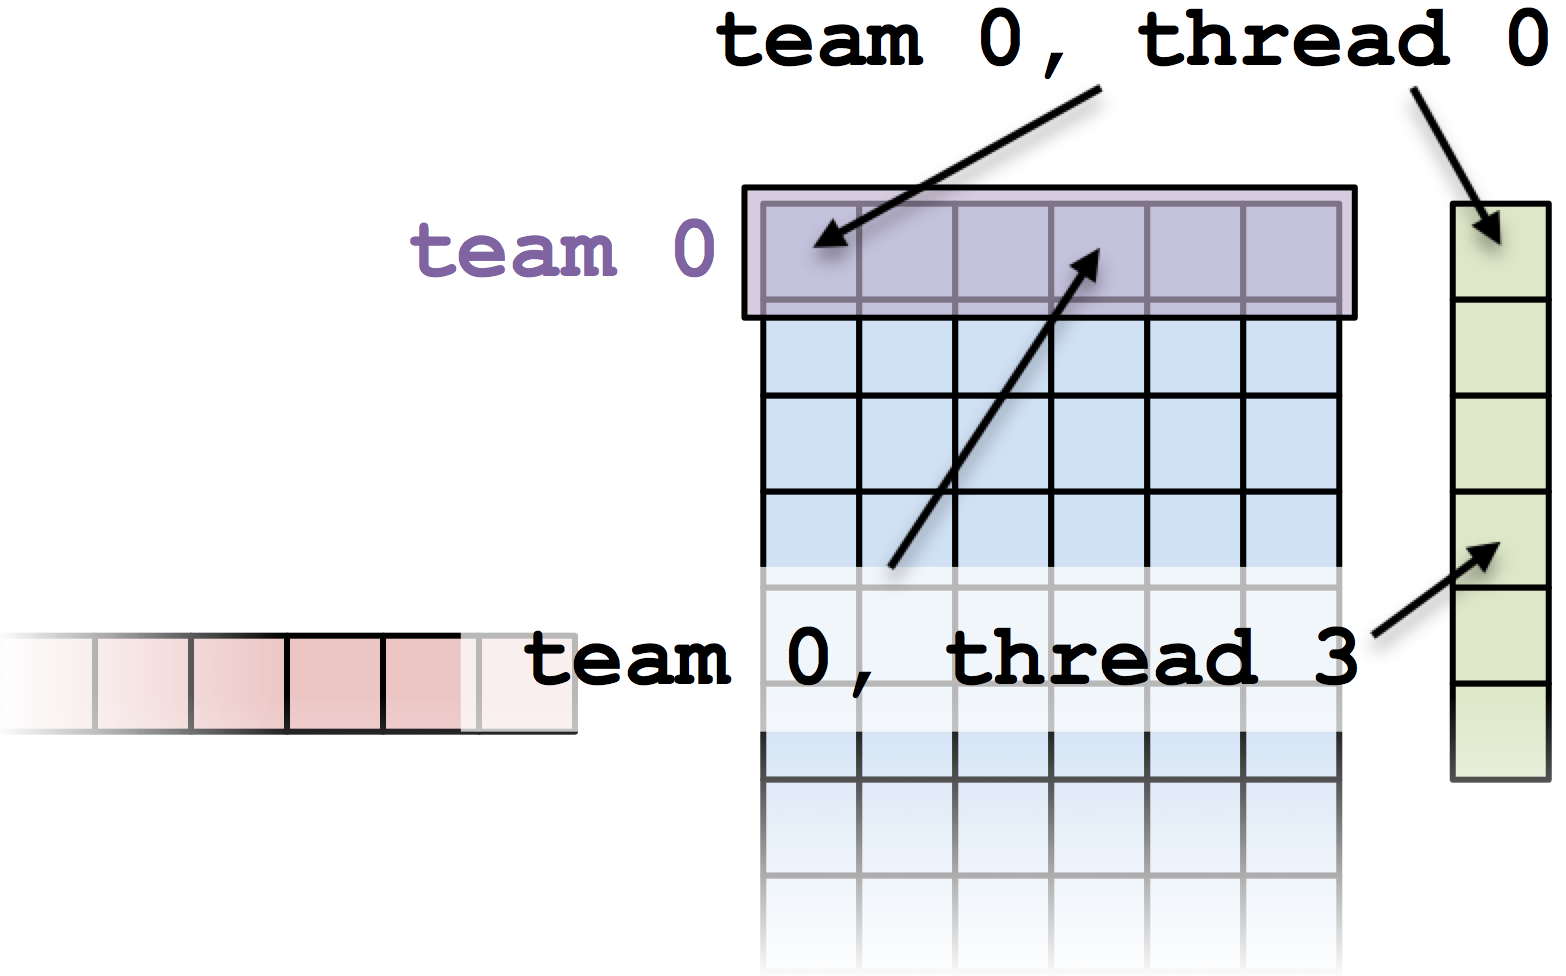
\includegraphics[width=0.53\textwidth]{figures/InnerProductExample_Teams}
      \end{tikzpicture}
      };
  \end{tikzpicture}

  High-level \textbf{strategy}:

  \vspace{-3pt}

  \begin{enumerate}
    \item{Do \textbf{one parallel launch} of \texttt{N} teams.}
    \item{Each team handles a row.}
    \item{The threads within \textbf{teams perform a reduction}.}
    \item{The thread teams \textbf{perform a reduction}.}
  \end{enumerate}

  %\vspace{-15pt}
  \vspace{85pt}

  %\begin{center}
    %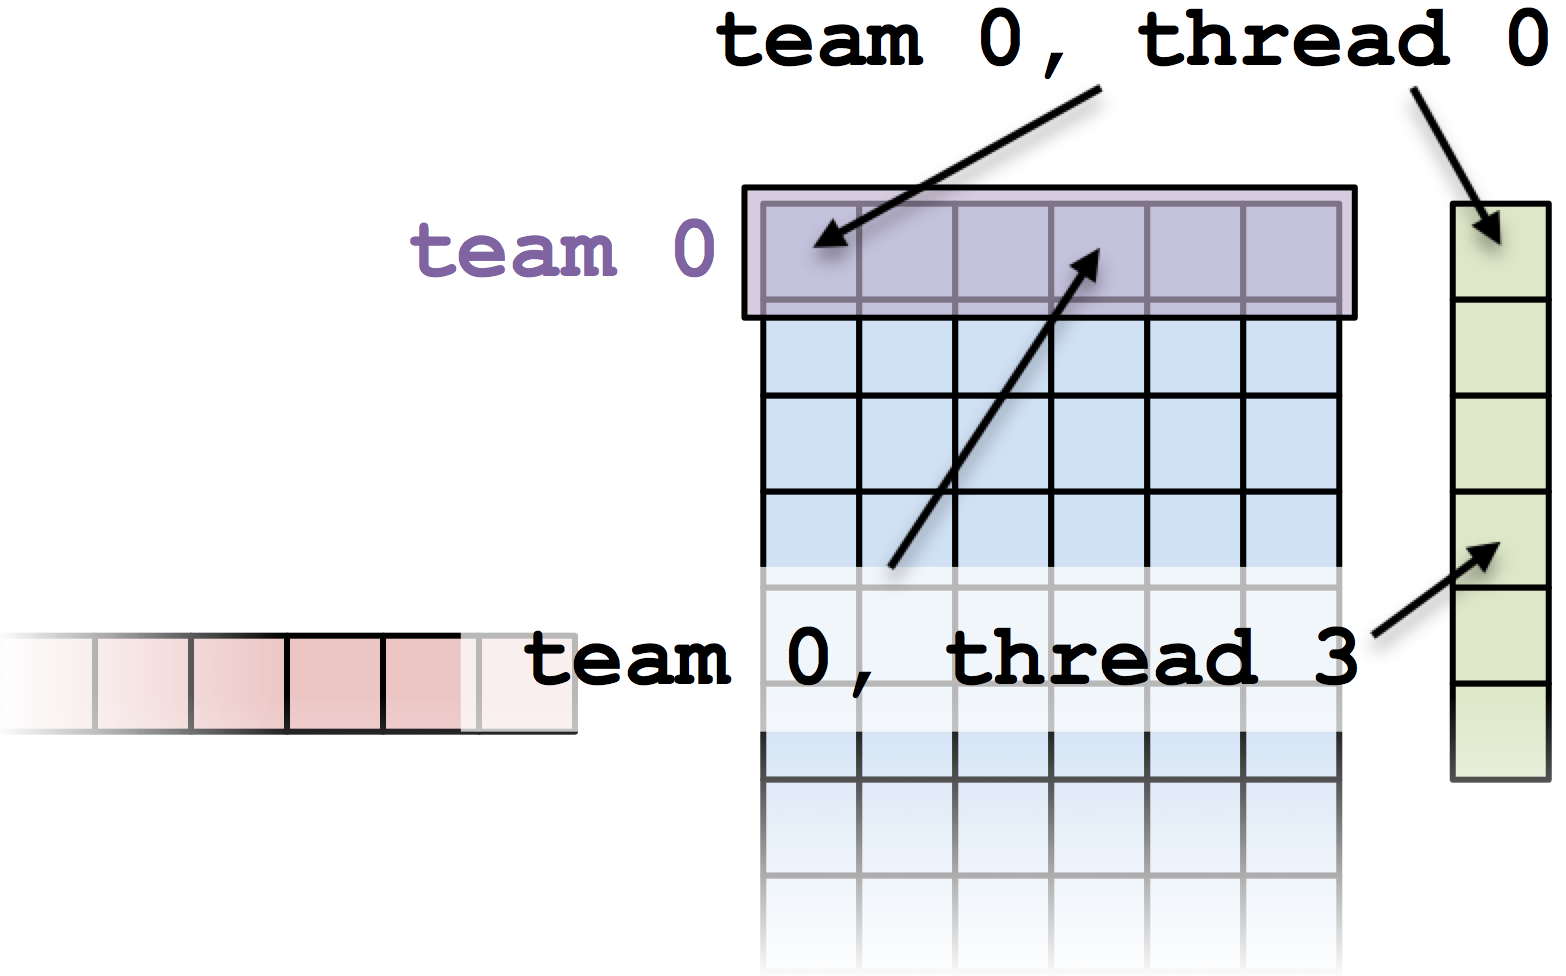
\includegraphics[width=0.40\textwidth]{figures/InnerProductExample_Teams}
  %\end{center}

  %\vspace{-5pt}

\end{frame}
\fi

%==========================================================================

\ifmedium
\begin{frame}[fragile]{Example: inner product (4)}

  \ul{\textbf{The \textit{final} hierarchical parallel kernel:}}

  \begin{code}
parallel_reduce("yAx",
  team_policy(N, Kokkos::AUTO),

  KOKKOS_LAMBDA (const member_type & @blueteamMember@blue, double & @orangeupdate@orange) {
    int @purplerow@purple = @blueteamMember@blue.league_rank();

    double thisRowsSum = 0;
    parallel_reduce(TeamThreadRange(@blueteamMember@blue, M),
      [=] (int @darkgreencol@darkgreen, double & @redinnerUpdate@red) {
        @redinnerUpdate@red += A(@purplerow@purple, @darkgreencol@darkgreen) * x(@darkgreencol@darkgreen);
      }, thisRowsSum);

    if (@blueteamMember@blue.team_rank() == 0) {
      update += y(@purplerow@purple) * thisRowsSum;
    }
  }, @orangeresult@orange);
  \end{code}

  %\vspace{5pt}

  %The \textbf{performance} and \textbf{flexibility} of teams is \emph{naturally} and \emph{concisely} expressed under the Kokkos model.

  %\vspace{1em}

  %Let's walk through how we got to this \textit{final} answer.

\end{frame}
\fi

%==========================================================================

\begin{frame}[fragile]{TeamPolicy (0)}

  \begin{block}{Important point}
    Using teams is changing the execution \emph{policy}.
  \end{block}

  \vspace{10pt}

  ``\textbf{Flat} parallelism'' uses \texttt{RangePolicy}:

  \vspace{3pt}

  \hspace{20pt}We specify a \emph{total amount of work}.

  \vspace{0pt}

  \begin{code}
// total work = N
@patternparallel_for@pattern("Label", 
  @policyRangePolicy<ExecutionSpace>(0,N)@policy, @bodyfunctor@body);
  \end{code}

  \pause
  \vspace{15pt}
  ``\textbf{Hierarchical} parallelism'' uses \texttt{TeamPolicy}:

  \vspace{3pt}

  \hspace{20pt}We specify a \emph{team size} and a \emph{number of teams}.

  \begin{code}[linebackgroundcolor={
      },
      keywords={}
    ]
// total work = numberOfTeams * teamSize
@patternparallel_for@pattern("Label", 
  @policyTeamPolicy<ExecutionSpace>(numberOfTeams, teamSize)@policy, @bodyfunctor@body);
  \end{code}

  \vspace{10pt}
\end{frame}

%==========================================================================

\begin{frame}[fragile]{TeamPolicy (1)}

  \begin{block}{Important point}
    When using teams, functor operators receive a \emph{team member}.
  \end{block}

  \begin{code}[linebackgroundcolor={
      },
      keywords={}
    ]
using member_type = typename TeamPolicy<ExecSpace>::member_type;

void operator()(const member_type & teamMember) {
  <@{\bf // How many teams are there?}@>
  const unsigned int league_size = teamMember.league_size();

  <@{\bf // Which team am I on?}@>
  const unsigned int league_rank = teamMember.league_rank();

  <@{\bf // How many threads are in the team?}@>
  const unsigned int team_size = teamMember.team_size();

  <@{\bf // Which thread am I on this team?}@>
  const unsigned int team_rank = teamMember.team_rank();

  <@{\bf // Make threads in a team wait on each other:}@>
  teamMember.team_barrier();
}
  \end{code}

\end{frame}


%==========================================================================

\iffull
\begin{frame}[fragile]{\texttt{TeamThreadRange} (0)}

 \begin{tikzpicture}[remember picture, overlay]
    \node [shift={(-6.0cm,-4.70cm)}]  at (current page.north east)
      {%
      \begin{tikzpicture}[remember picture, overlay]
        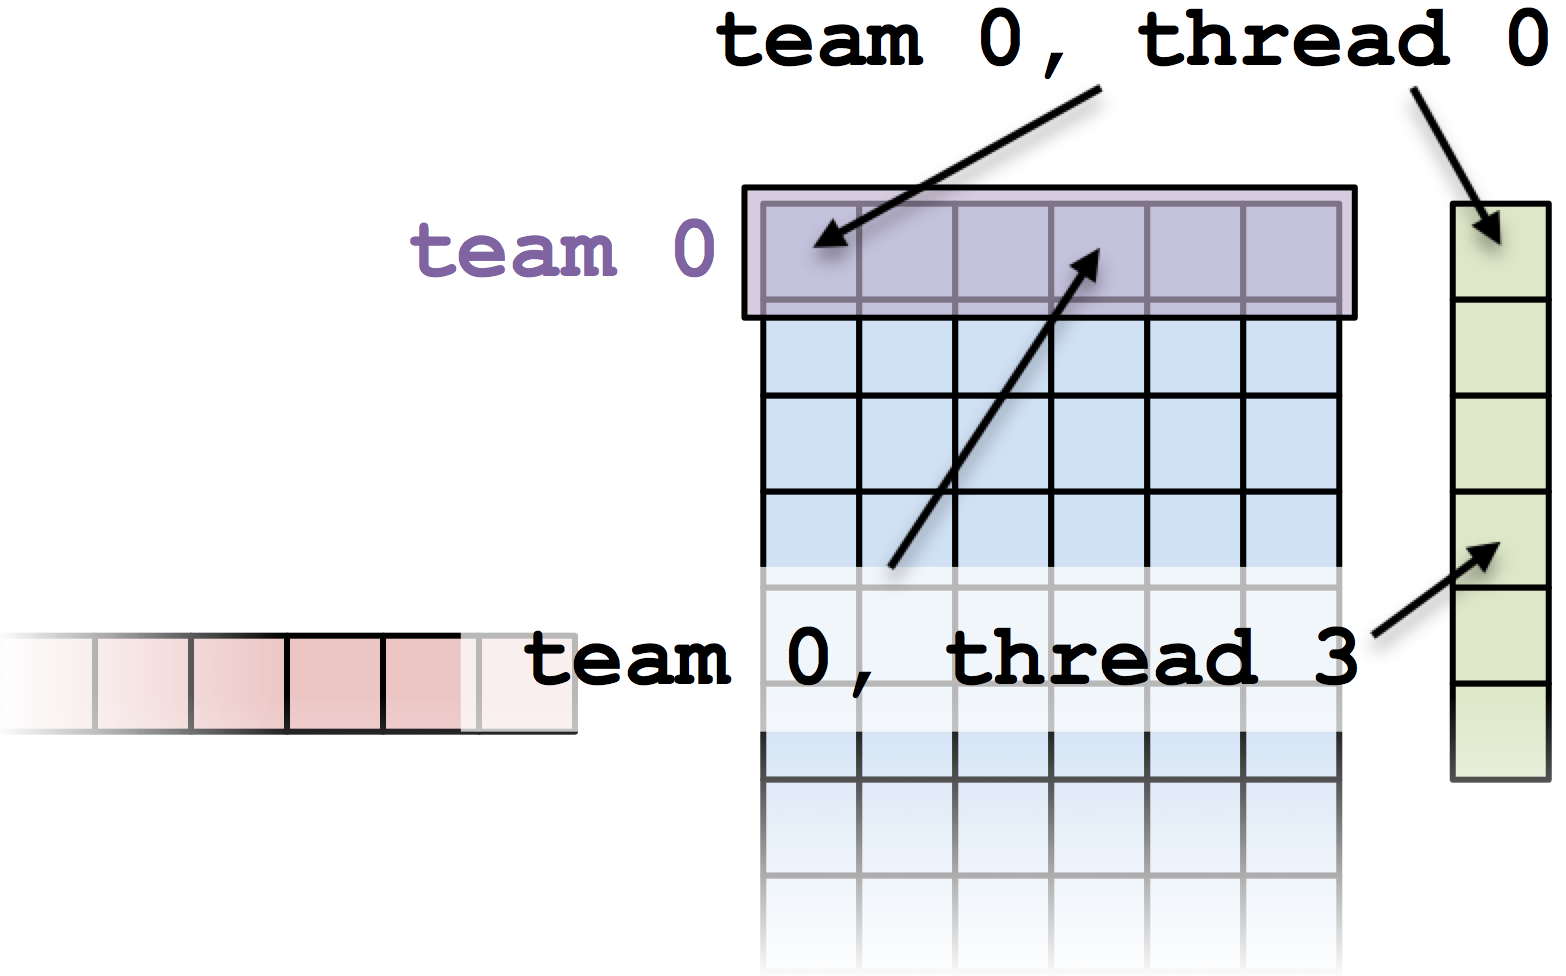
\includegraphics[width=0.53\textwidth]{figures/InnerProductExample_Teams}
      \end{tikzpicture}
      };
  \end{tikzpicture}

  \vspace{50pt}

  First attempt at exercise:

  \begin{code}
@grayoperator() (member_type & teamMember ) {
  const size_t row = teamMember.league_rank();
  const size_t col = teamMember.team_rank();@gray
  atomic_add(&@orangeresult@orange,@darkredy@darkred(row) * @blueA@blue(row,col) * @darkgreenx@darkgreen(entry));
@gray}@gray
  \end{code}

  \pause
  \vspace{-5pt}

  \begin{itemize}

  \item {When team size $\neq$ number of columns, how are units of work mapped to team's member threads?  Is the mapping architecture-dependent?}

  \end{itemize}

\end{frame}
\fi

%==========================================================================

\iffull
\begin{frame}[fragile]{\texttt{TeamThreadRange} (1)}


  Second attempt at exercise:

\vspace{10pt}
  Divide row length among team members.

  \begin{code}
@grayoperator() (member_type & teamMember ) {
  const size_t row = teamMember.league_rank();

  int begin = teamMember.team_rank();
  for(int col = begin; col < M; col += teamMember.team_size()) {
    atomic_add(&@orangeresult@orange, @darkredy@darkred(row) * @blueA@blue(row,col) * @darkgreenx@darkgreen(entry));
  }
@gray}@gray
  \end{code}

  \pause
  \vspace{-5pt}

  \begin{itemize}

  \item {Still bad because \texttt{atomic\_add} performs badly under high contention, how can team's member threads performantly cooperate for a nested reduction?}

  \item {On CPUs you get a bad data access pattern: this hardcodes coalesced access, but not caching.}

  \end{itemize}

\end{frame}
\fi

%==========================================================================

\begin{frame}[fragile]{\texttt{TeamThreadRange} (2)}

  We shouldn't be hard-coding the work mapping...

  \begin{code}[linebackgroundcolor={
        \btLstHL<1->{6}{bodyColor}
      },
      keywords={}
    ]
@grayoperator() (member_type & teamMember, double & update) {
  const int row = teamMember.league_rank();@gray
  double @purplethisRowsSum@purple;
  @pattern``do a reduction''@pattern(@policy``over M columns''@policy,
    [=] (const int col) {
      @purplethisRowsSum@purple += @blueA@blue(row,col) * @darkgreenx@darkgreen(col);
    });
  if (teamMember.team_rank() == 0) {
    update += @darkred@darkred(row) * @purplethisRowsSum@purple;
  }
@gray}@gray
  \end{code}

  \pause
  \vspace{5pt}

  If this were a parallel execution, \\
    \hspace{20pt}we'd use \texttt{Kokkos::parallel\_reduce}.

  \pause
  \vspace{5pt}

  \textbf{Key idea}: this \emph{is} a parallel execution.

  \pause
  \vspace{5pt}

  \hspace{20pt}{\Large $\Rightarrow$ \textbf{Nested parallel patterns}}

\end{frame}

%==========================================================================

\begin{frame}[fragile]{\texttt{TeamThreadRange} (3)}

  \ul{\texttt{TeamThreadRange}:}

  \begin{code}[linebackgroundcolor={
        \btLstHL<1->{6}{bodyColor}
      },
      keywords={}
    ]
@grayoperator() (const member_type & teamMember, double & update ) {
  const int row = teamMember.league_rank();@gray
  double @purplethisRowsSum@purple;
  @patternparallel_reduce@pattern(@policyTeamThreadRange(teamMember, M)@policy,
    [=] (const int col, double & thisRowsPartialSum ) {
      thisRowsPartialSum += @blueA@blue(row, col) * @darkgreenx@darkgreen(col);
    }, @purplethisRowsSum@purple );
  if (teamMember.team_rank() == 0) {
    update += @darkredy@darkred(row) * @purplethisRowsSum@purple;
  }
@gray}@gray
  \end{code}

  \pause

  \begin{itemize}
    \item{The \textbf{mapping} of work indices to threads is \textbf{architecture-dependent}.}
    \item{The \textbf{amount of work} given to the \texttt{TeamThreadRange} \textbf{need not be a multiple} of the \texttt{team\_size}.}
    \item{Intrateam \textbf{reduction handled} by Kokkos.}
  \end{itemize}

\end{frame}

%==========================================================================

\begin{frame}[fragile]{Nested parallelism}

  \ul{\textbf{Anatomy} of nested parallelism:}

  \vspace{-3pt}

  \begin{code}[linebackgroundcolor={
        %\btLstHL<1->{4-7}{bodyColor}
      },
      keywords={}
    ]
@patternparallel_outer@pattern("Label",
  @policyTeamPolicy<ExecutionSpace>(numberOfTeams, teamSize)@policy,
  KOKKOS_LAMBDA (const member_type & teamMember@italic[, ...]@italic) {
    /* beginning of outer body */
    @patternparallel_inner@pattern(
      @policyTeamThreadRange(teamMember, thisTeamsRangeSize)@policy,
      [=] (const unsigned int indexWithinBatch@italic[, ...]@italic) {
        /* inner body */
      }@italic[, ...]@italic);
    /* end of outer body */
  }@italic[, ...]@italic);
  \end{code}

  \vspace{-5pt}

  \begin{itemize}
    \item{\texttt{parallel\_outer} and \texttt{parallel\_inner} may be any combination of \texttt{for} and/or \texttt{reduce}.}
    \item{The inner lambda may capture by reference, but capture-by-value is recommended.}
    \item{The policy of the inner lambda is always a \texttt{TeamThreadRange}.}
    \item{\texttt{TeamThreadRange} cannot be nested.}
  \end{itemize}

\end{frame}

%==========================================================================

\begin{frame}[fragile]{What should the team size be?}

  In practice, you can \textbf{let Kokkos decide}:

    \begin{code}[linebackgroundcolor={
      },
      keywords={}
    ]
parallel_something(
  TeamPolicy<ExecutionSpace>(numberOfTeams, Kokkos::AUTO),
  /* functor */);
    \end{code}

  \pause
  \vspace{0pt}

  \ul{\textbf{GPUs}}

  \begin{itemize}
    \item{Special hardware available for coordination within a team.}
    \item{Within a team 32 (NVIDIA) or 64 (AMD) threads execute ``lock step.''}
    \item{Maximum team size: \textbf{1024}; Recommended team size: \textbf{128/256}}
  \end{itemize}

  \pause
  \vspace{0pt}

  \ul{\textbf{Intel Xeon Phi}:}

  \begin{itemize}
    \item{Recommended team size: \# hyperthreads per core}
    \item{Hyperthreads share entire cache hierarchy} \\
      \hspace{2em}{a well-coordinated team avoids cache-thrashing}
  \end{itemize}

\end{frame}

%==========================================================================

\begin{frame}[fragile]{Exercise: TeamPolicy}

  \textbf{Details}:
  \begin{small}
  \begin{itemize}
\item Location: \ExerciseDirectory{team\_policy}
\item Replace \texttt{RangePolicy<Space>} with \texttt{TeamPolicy<Space>}
\item Use \texttt{AUTO} for \texttt{team\_size}
\item Make the inner loop a \texttt{parallel\_reduce} with \texttt{TeamThreadRange} policy
\item Experiment with the combinations of \texttt{Layout}, \texttt{Space}, \texttt{N} to view performance
\item Hint: what should the layout of \texttt{A} be?
\end{itemize}
  \end{small}

\ul{\textbf{Things to try:}}
  \begin{small}
  \begin{itemize}
  \item Vary problem size and number of rows (-S ...; -N ...)
  \item Compare behavior with Exercise 4 for very non-square matrices
  \item Compare behavior of CPU vs GPU
  \end{itemize}
  \end{small}

\end{frame}

%==========================================================================

\begin{frame}[fragile]{Reminder, Exercise \#4 with Flat Parallelism}

  \vspace{-10pt}

    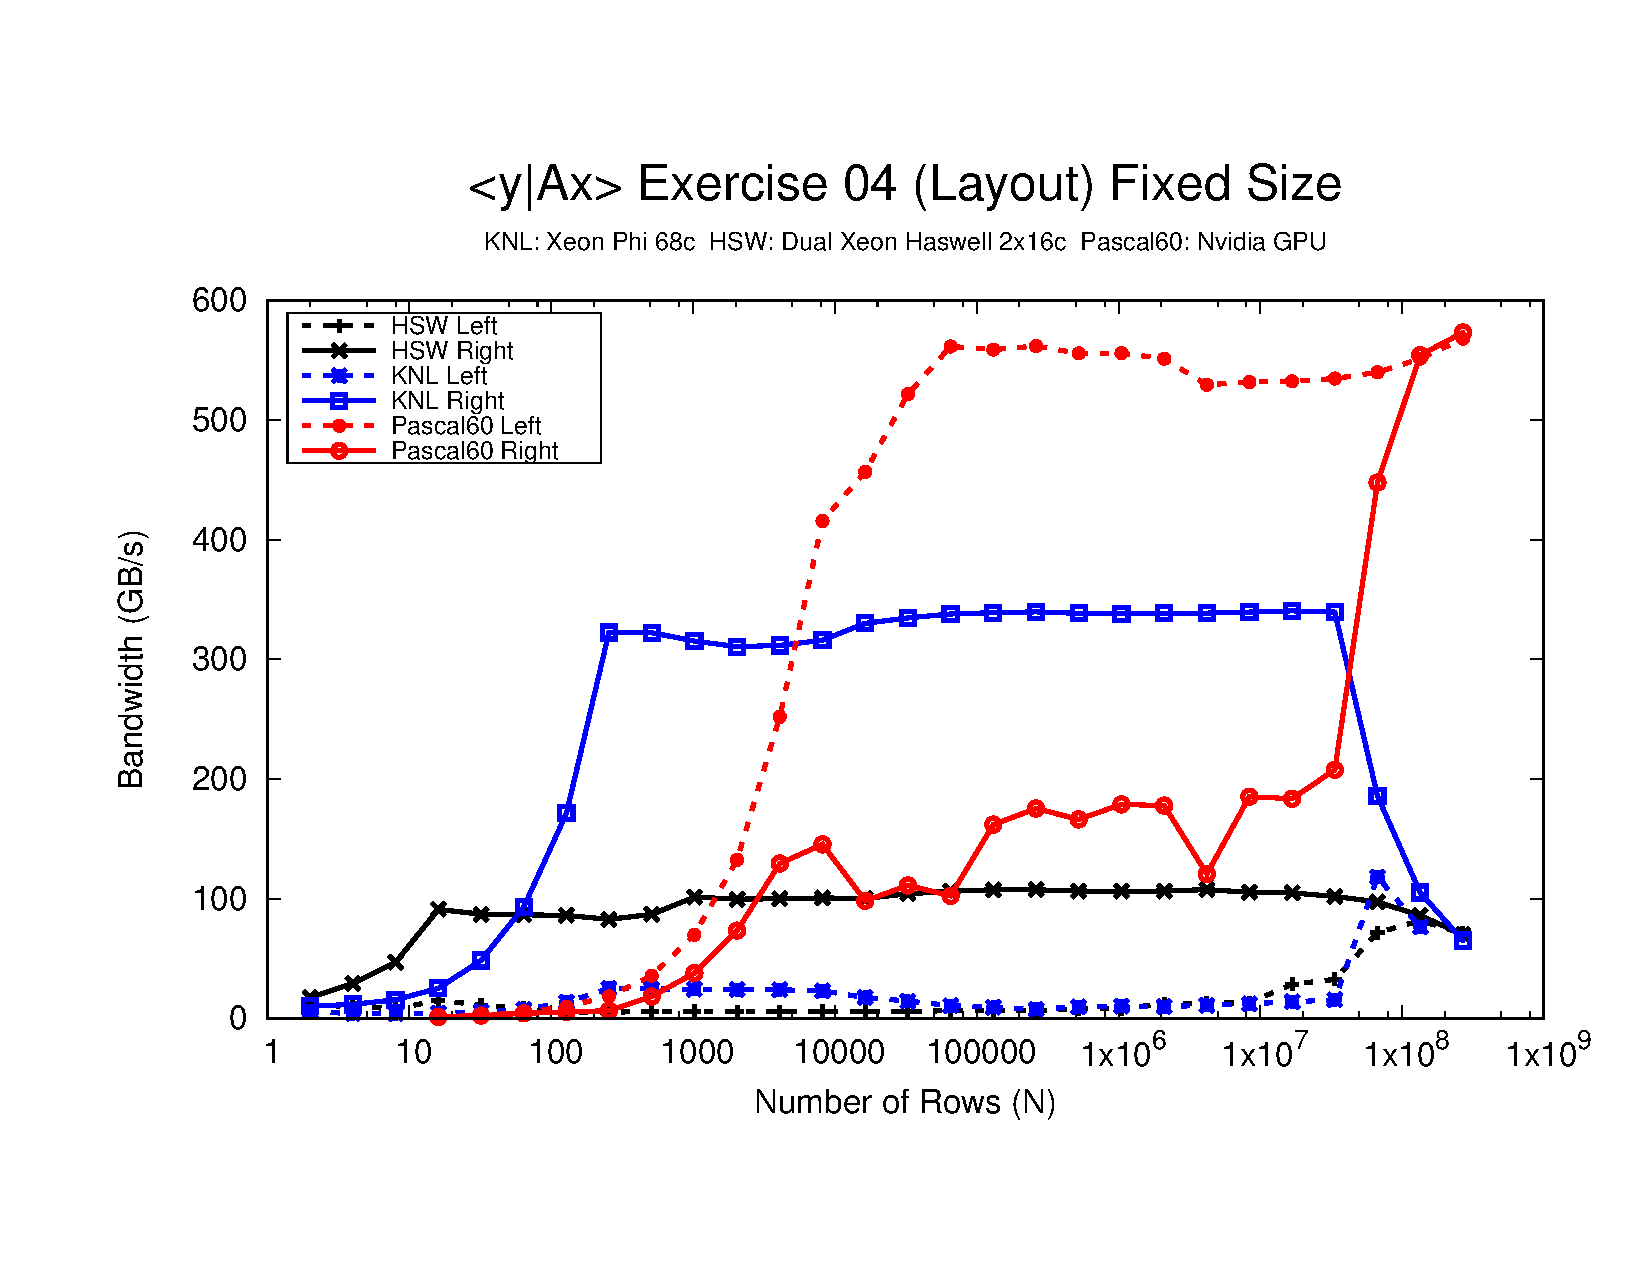
\includegraphics[viewport=1.25in 3.0in 10in 6in, width=0.95\textwidth]{figures/Exercise04-Performance.pdf}

  \vspace{-15pt}

  \begin{textblock*}{0.5\textwidth}(0.65\textwidth,0.28\textheight)
    \textbf{coalesced}
  \end{textblock*}

  \begin{textblock*}{0.5\textwidth}(0.60\textwidth,0.44\textheight)
    \textbf{cached}
  \end{textblock*}

  \begin{textblock*}{0.5\textwidth}(0.60\textwidth,0.61\textheight)
    \textbf{uncoalesced}
  \end{textblock*}

  \begin{textblock*}{0.5\textwidth}(0.70\textwidth,0.68\textheight)
    \textbf{cached}
  \end{textblock*}

  \begin{textblock*}{0.5\textwidth}(0.70\textwidth,0.77\textheight)
    \textbf{uncached}
  \end{textblock*}

\end{frame}

%==========================================================================

\begin{frame}[fragile]{Exercise: TeamPolicy}

  \vspace{-10pt}

  \begin{center}
    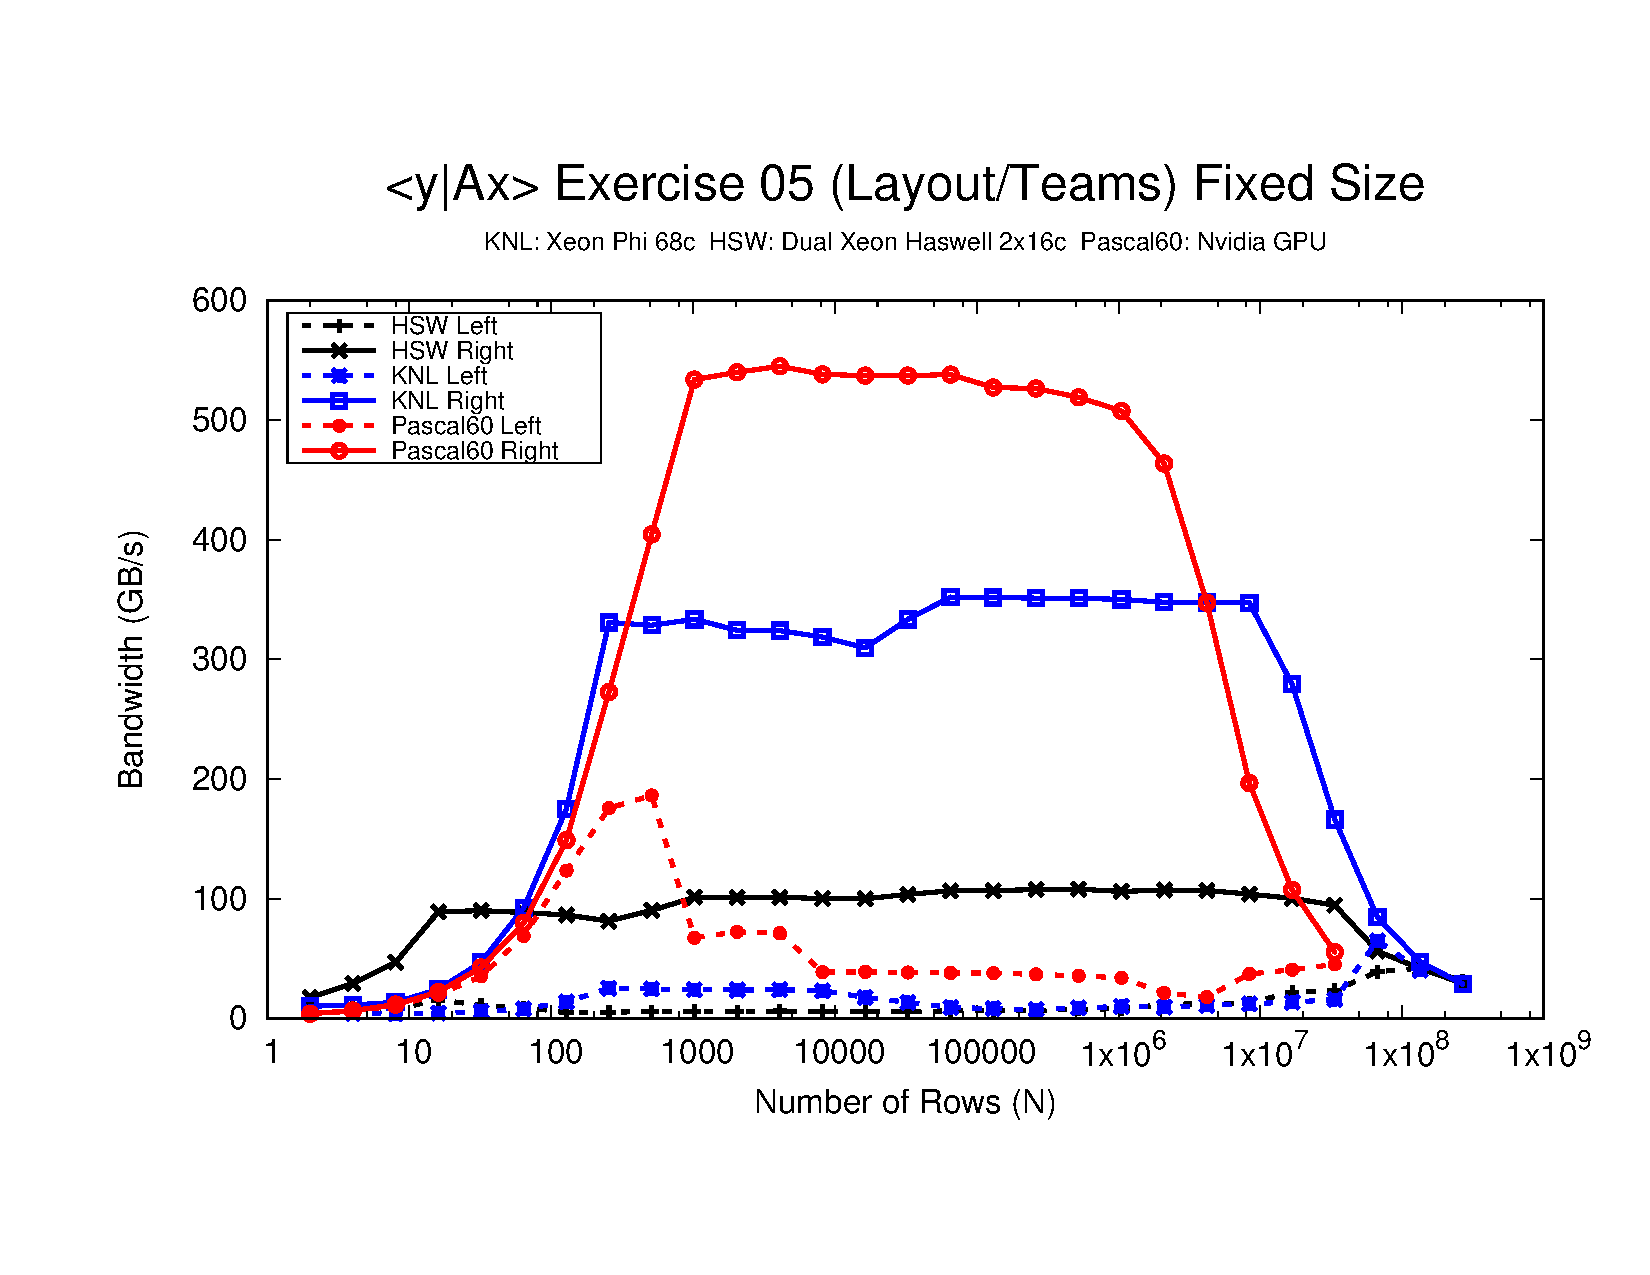
\includegraphics[viewport=1.25in 3.0in 10in 6in, width=0.95\textwidth]{figures/Exercise05-Performance.pdf}
  \end{center}

  \vspace{-15pt}

  \begin{textblock*}{0.5\textwidth}(0.55\textwidth,0.32\textheight)
    \textbf{coalesced}
  \end{textblock*}

  \begin{textblock*}{0.5\textwidth}(0.60\textwidth,0.44\textheight)
    \textbf{cached}
  \end{textblock*}

  \begin{textblock*}{0.5\textwidth}(0.70\textwidth,0.68\textheight)
    \textbf{cached}
  \end{textblock*}

\end{frame}

%==========================================================================

\begin{comment}
\begin{frame}[fragile]{Example: sparse matrix-vector product (0)}

  Sparse matrix \textbf{representation}:

  \vspace{-7pt}

  \begin{table}
    \small
    \begin{tabular}{| l | c | c | c | c | c |}
      \hline
      \texttt{colIndices} & 17 & 45 & 73 & 7 & ... \\
      \hline
      \texttt{colValues} & 3.1 & 4.1 & 5.9 & 2.6 & ...\\
      \hline
      \texttt{irow} & 0 & 3 & 9 & ... & \\
      \hline
    \end{tabular}
  \end{table}

  \vspace{10pt}

  \textbf{Serial} algorithm:

  \vspace{-2pt}

  \begin{code}[linebackgroundcolor={
      },
      keywords={}
    ]
for (row = 0; row < matrixSize; ++row) {
  double total = 0;
  for (int i = irow[row]; i < irow[row+1]; ++i) {
    total += colValues[i] * vec[colIndices[i]];
  }
  product[row] = total;
}
  \end{code}

  \pause
  \vspace{10pt}

  How many ways can this be parallelized?

\end{frame}

%==========================================================================

\begin{frame}[fragile]{Example: sparse matrix-vector product (1)}

  \ul{\textbf{Flat} over \textbf{rows}:}

  \begin{code}[linebackgroundcolor={
      },
      frame=single,
      keywords={}
    ]
operator()(int row) const {
  double total = 0;
  for (int i = _irow(row); i < _irow(row+1); ++i) {
    total += _colValues(i) * _vec(_colIndices(i));
  }
  _product[row] = total;
}
  \end{code}

  \vspace{5pt}

  \begin{itemize}
    \item{One thread \textbf{per row}}
    \item{\texttt{\_colValues} and \texttt{\_colIndices}: {\color{darkgreen}cached}/{\color{darkred}uncoalesced}}
    \item{\texttt{\_vec}: {\color{darkred}uncached}/{\color{darkred}uncoalesced}}
    \item{\texttt{\_product}: {\color{darkgreen}cached}/{\color{darkgreen}coalesced}}
  \end{itemize}

\end{frame}

%==========================================================================

\begin{frame}[fragile]{Example: sparse matrix-vector product (2)}

  \ul{\textbf{Flat} over \textbf{non-zeros} with atomics:}

  \begin{code}[linebackgroundcolor={
      },
      frame=single,
      keywords={}
    ]
operator()(int i) const {
  atomic_add(&_product(_rowIndices(i)),
             colValues(i) * _vec(_colIndices(i)));
}
  \end{code}

  \begin{itemize}
    \item{One thread \textbf{per nonzero entry}}
    \item{\texttt{\_colValues}, \texttt{\_colIndices}, \texttt{\_rowIndices}: {\color{darkgreen}cached}/{\color{darkgreen}coalesced}}
    \item{\texttt{\_vec}: {\color{darkred}uncached}/{\color{darkred}uncoalesced}}
    \item{\texttt{\_product}: {\color{darkgreen}good}/{\color{darkred}bad}}
  \end{itemize}

\end{frame}

%==========================================================================

\begin{frame}[fragile]{Example: sparse matrix-vector product (3)}

  \ul{Hierarchical \textbf{thread teams}:}

  \begin{code}[linebackgroundcolor={
      },
      frame=single,
      keywords={}
    ]
operator()(member_type teamMember) const {
  int row = teamMember.league_rank();
  double total;
  Kokkos::parallel_reduce
    (Kokkos::TeamThreadRange(teamMember, numNonzeros),
     [=] (const unsigned int j, double & valueToUpdate) {
      const unsigned int i = irow(row) + j;
      valueToUpdate += _colValues(i) * _vec(_colIndices(i));
    }, total);
  if (teamMember.team_rank() == 0) {
    _product(row) = total;
  }
}
  \end{code}

  \vspace{-5pt}

  \begin{itemize}
    \item{One thread \textbf{per nonzero entry}}
    \item{\texttt{\_colValues}, \texttt{\_colIndices}: {\color{darkgreen}cached}/{\color{darkgreen}coalesced}}
    \item{\texttt{\_vec}: {\color{darkred}uncached}/{\color{darkred}uncoalesced}}
    \item{\texttt{\_product}: {\color{darkgreen}cached}/{\color{darkgreen}single write}}
  \end{itemize}

\end{frame}

%==========================================================================

\begin{frame}[fragile]{Example: sparse matrix-vector product (4)}

  \ul{\textbf{Performance:}}

  \begin{center}
    \includegraphics[width=1.00\textwidth]{figures/SparseMatrixVectorProduct_summaryNoTexture.pdf}
  \end{center}

\end{frame}

%==========================================================================

\begin{frame}[fragile]{Example: sparse matrix-vector product (5)}

  \ul{\textbf{Performance} (including texture versions):}

  \begin{center}
    \includegraphics[width=1.00\textwidth]{figures/SparseMatrixVectorProduct_summary.pdf}
  \end{center}

\end{frame}
\end{comment}

%==========================================================================

\begin{frame}[fragile]{Three-level parallelism (0)}

  \ul{\textbf{Exposing Vector Level Parallelism}}

  \begin{itemize}
    \item{Optional \textbf{third level} in the hierarchy: \texttt{ThreadVectorRange}}
      \begin{itemize}
        \item{Can be used for \texttt{parallel\_for}, \texttt{parallel\_reduce}, or \texttt{parallel\_scan}.}
      \end{itemize}
    \item{Maps to vectorizable loop on CPUs or (sub-)warp level parallelism on GPUs.}
    \item{Enabled with a \textbf{runtime} vector length argument to \texttt{TeamPolicy}}
    \item{There is \textbf{no} explicit access to a vector lane ID.}
    \item{Depending on the backend the full global parallel region has active vector lanes.}
    \item{\texttt{TeamVectorRange} uses both \textbf{thread} and \textbf{vector} parallelism.}
  \end{itemize}


\end{frame}

%==========================================================================

\begin{frame}[fragile]{Three-level parallelism (1)}

  \ul{\textbf{Anatomy} of nested parallelism:}

  \vspace{-3pt}

  \begin{code}[linebackgroundcolor={
        %\btLstHL<1->{4-7}{bodyColor}
      },
      keywords={}
    ]
@patternparallel_outer@pattern("Label",
  @policyTeamPolicy<>(numberOfTeams, teamSize, vectorLength)@policy,
  KOKKOS_LAMBDA (const member_type & teamMember@italic[, ...]@italic) {
    /* beginning of outer body */
    @patternparallel_middle@pattern(
      @policyTeamThreadRange(teamMember, thisTeamsRangeSize)@policy,
      [=] (const int indexWithinBatch@italic[, ...]@italic) {
        /* begin middle body */
        @patternparallel_inner@pattern(
           @policyThreadVectorRange(teamMember, thisVectorRangeSize)@policy,
           [=] (const int indexVectorRange@italic[, ...]@italic) {
             /* inner body */
           }@italic[, ....);
        /* end middle body */
      }@italic[, ...]@italic);
    @patternparallel_middle@pattern(
    @policyTeamVectorRange(teamMember, someSize)@policy,
      [=] (const int indexTeamVector[, ...]) {
	/* nested body */
      }[, ...]);
    /* end of outer body */
  }@italic[, ...]@italic);
  \end{code}

\end{frame}

%==========================================================================

\ifmedium
\begin{frame}[fragile]{Sum sanity checks (0)}

  \textbf{Question:} What will the value of \texttt{totalSum} be?

  \begin{code}[linebackgroundcolor={}]
int @darkgreentotalSum@darkgreen = 0;
parallel_reduce("Sum", RangePolicy<>(0, numberOfThreads),
  KOKKOS_LAMBDA (size_t& index, int& @darkredpartialSum@darkred) {
    int @bluethisThreadsSum@blue = 0;
    for (int i = 0; i < 10; ++i) {
      ++@bluethisThreadsSum@blue;
    }
    @darkredpartialSum@darkred += @bluethisThreadsSum@blue;
}, @darkgreentotalSum@darkgreen);
  \end{code}

  \pause

  \vspace{15pt}

  \texttt{totalSum = numberOfThreads * 10}

\end{frame}
\fi

%==========================================================================

\ifmedium
\begin{frame}[fragile]{Sum sanity checks (1)}

  \textbf{Question:} What will the value of \texttt{totalSum} be?

  \begin{code}[linebackgroundcolor={}]
@grayint totalSum = 0;
parallel_reduce("Sum", @grayTeamPolicy<>(numberOfTeams, team_size),
  @grayKOKKOS_LAMBDA (@graymember_type& teamMember,@gray int& partialSum) {
    int thisThreadsSum = 0;
    for (int i = 0; i < 10; ++i) {
      ++thisThreadsSum;
    }
    partialSum += thisThreadsSum;
}, totalSum);@gray
  \end{code}

  \pause

  \vspace{15pt}

  \texttt{totalSum = numberOfTeams * team\_size * 10}

\end{frame}
\fi

%==========================================================================

\ifmedium
\begin{frame}[fragile]{Sum sanity checks (2)}

  \textbf{Question:} What will the value of \texttt{totalSum} be?

  \begin{code}[linebackgroundcolor={}]
@grayint totalSum = 0;
parallel_reduce("Sum", TeamPolicy<>(numberOfTeams, team_size),
  KOKKOS_LAMBDA (member_type& teamMember, int& partialSum) {@gray
    int @orangethisTeamsSum@orange = 0;
    parallel_reduce(TeamThreadRange(teamMember, team_size),
      [=] (const int index, int& @purplethisTeamsPartialSum@purple) {
      @grayint thisThreadsSum = 0;
      for (int i = 0; i < 10; ++i) {
        ++thisThreadsSum;
      }@gray
      @purplethisTeamsPartialSum@purple += thisThreadsSum;
    }, @orangethisTeamsSum@orange);
    partialSum += @orangethisTeamsSum@orange;
@gray}, totalSum);@gray
  \end{code}

  \pause

  \vspace{15pt}

  \texttt{totalSum = numberOfTeams * team\_size * team\_size * 10}

\end{frame}
\fi

%==========================================================================

\begin{frame}[fragile]{Restricting Execution: single pattern}
The \texttt{single} pattern can be used to restrict execution
 \begin{itemize}
    \item{Like parallel patterns it takes a policy, a lambda, and optionally a broadcast argument.}
    \item{Two policies: \texttt{PerTeam} and \texttt{PerThread}.}
    \item{Equivalent to OpenMP {\bf single} directive with {\bf nowait}}
 \end{itemize}
\begin{code}[linebackgroundcolor={}]
// Restrict to once per thread
single(PerThread(teamMember), [&] () {
  // code
});

// Restrict to once per team with broadcast
int broadcastedValue = 0;
single(PerTeam(teamMember), [&] (int& broadcastedValue_local) {
	broadcastedValue_local = special value assigned by one;
}, broadcastedValue);
// Now everyone has the special value
\end{code}
\end{frame}

%==========================================================================

\begin{frame}[fragile]{Exercise: TeamVectorLoop}
The previous example was extended with an outer loop over ``Elements'' to expose
a third natural layer of parallelism.

\vspace{10pt}

  \textbf{Details}:
  \begin{small}
  \begin{itemize}
\item Location: \ExerciseDirectory{team\_vector\_loop}
\item Use the \texttt{single} policy instead of checking team rank
\item Parallelize all three loop levels.
\end{itemize}
  \end{small}

\ul{\textbf{Things to try:}}
  \begin{small}
  \begin{itemize}
  \item Vary problem size and number of rows (-S ...; -N ...)
  \item Compare behavior with TeamPolicy Exercise for very non-square matrices
  \item Compare behavior of CPU vs GPU
  \end{itemize}
  \end{small}
\end{frame}

%==========================================================================

\begin{frame}[fragile]{Exercise: TeamVectorLoop}

  %\vspace{-10pt}

    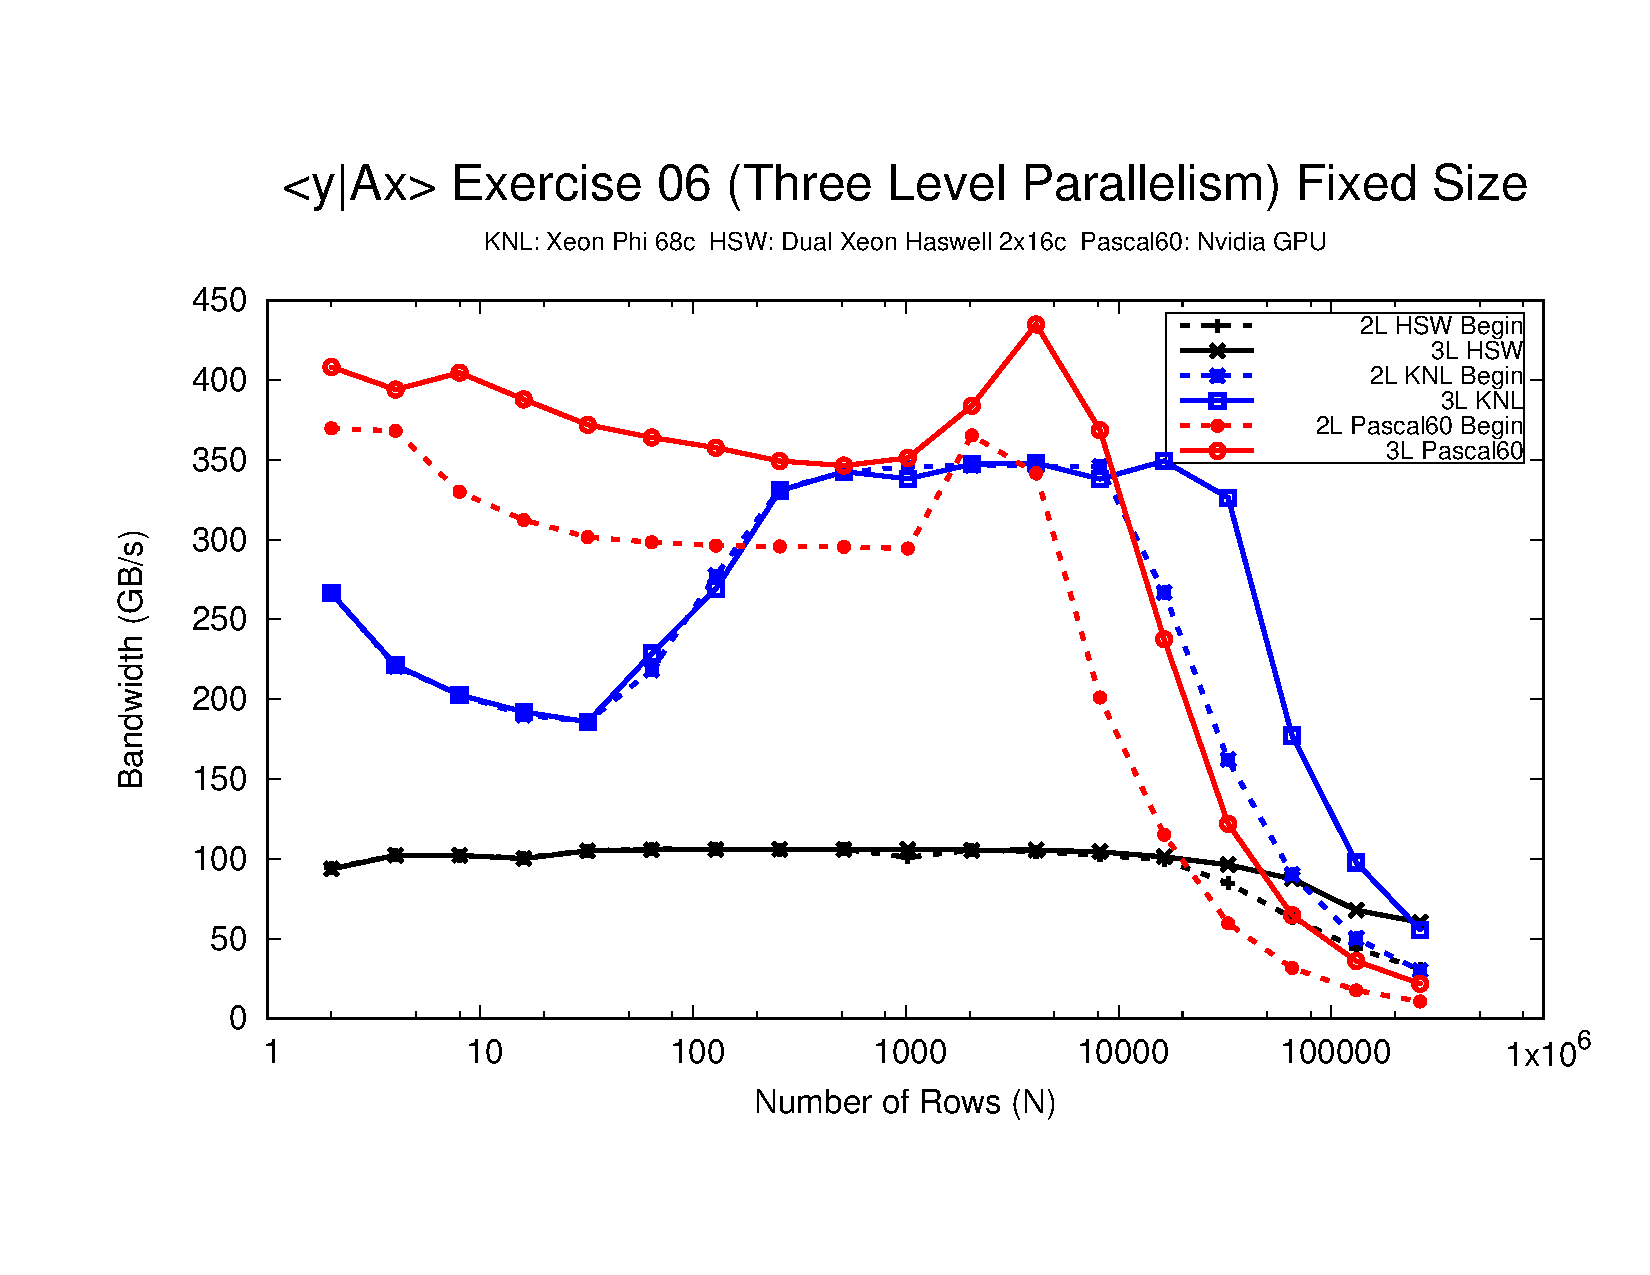
\includegraphics[viewport=1.25in 3.0in 10in 6in, width=0.95\textwidth]{figures/Exercise06-Performance.pdf}

  \vspace{-15pt}

\end{frame}

%==========================================================================

\begin{frame}{Section Summary}

  \begin{itemize}
    \item{\textbf{Hierarchical work} can be parallelized via hierarchical parallelism.}
    \item{Hierarchical parallelism is leveraged using \textbf{thread teams} launched with a \texttt{TeamPolicy}.}
    \item{Team ``worksets'' are processed by a team in nested \texttt{parallel\_for} (or \texttt{reduce} or \texttt{scan}) calls with a \texttt{TeamThreadRange}, \texttt{ThreadVectorRange}, and \texttt{TeamVectorRange} policy.}
    \item{Execution can be restricted to a subset of the team with the \texttt{single} pattern using either a \texttt{PerTeam} or \texttt{PerThread} policy.}
  \end{itemize}

\end{frame}

%==========================================================================

\begin{frame}[fragile]

  {\Huge Scratch memory}

  \vspace{20pt}

  \textbf{Learning objectives:}
  \begin{itemize}
    \item {Understand concept of \textbf{team} and \textbf{thread} private \textbf{scratch pads}}
    \item {Understand how scratch memory can \textbf{reduce global memory accesses}}
    \item {Recognize \textbf{when to use} scratch memory}
    \item {Understand \textbf{how to use} scratch memory and when barriers are necessary}
  \end{itemize}

  \vspace{-20pt}

\end{frame}

%==========================================================================

\begin{frame}[fragile]{Types of Scratch Space Uses}
\vspace{-8pt}
\textbf{Two Levels of Scratch Space}
\begin{itemize}
\item{Level 0 is limited in size but fast.}
\item{Level 1 allows larger allocations but is equivalent to High Bandwidth Memory in latency and bandwidth.}
\end{itemize}

\textbf{Team or Thread private memory}
\begin{itemize}
\item{Typically used for per work-item temporary storage.}
\item{Advantage over pre-allocated memory is aggregate size scales with number of threads, not number of work-items.}
\end{itemize}

\textbf{Manually Managed Cache}
\begin{itemize}
\item{Explicitly cache frequently used data.}
\item{Exposes hardware specific on-core scratch space (e.g. NVIDIA GPU Shared Memory).}
\end{itemize}

\pause
\vspace{2pt}
\textbf{Now: Discuss Manually Managed Cache Usecase.}
\end{frame}
%==========================================================================

\begin{frame}[fragile]{Example: contractDataFieldScalar (1)}

  \ul{\textbf{One slice of contractDataFieldScalar:}}

  \vspace{-10pt}

  \begin{center}
    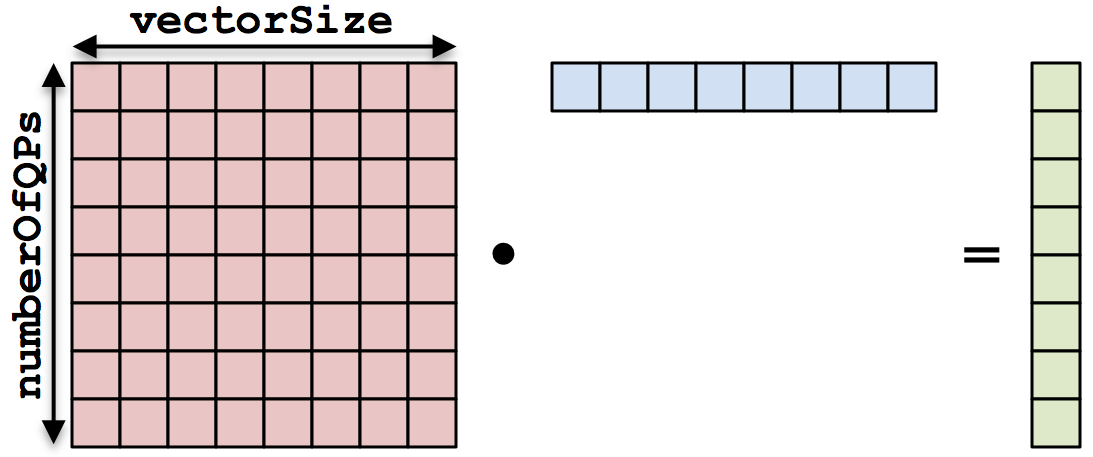
\includegraphics[width=0.65\textwidth]{figures/ContractDataFieldScalar_slice}
  \end{center}

  \begin{code}[frame=single, keywords={}]
for (qp = 0; qp < numberOfQPs; ++qp) {
  total = 0;
  for (i = 0; i < vectorSize; ++i) {
    total += @darkredA@darkred(qp, i) * @blueB@blue(i);
  }
  @darkgreenresult@darkgreen(qp) = total;
}
  \end{code}

\end{frame}

%==========================================================================

\begin{frame}[fragile]{Example: contractDataFieldScalar (2)}

  \ul{\textbf{contractDataFieldScalar:}}

  \vspace{-10pt}

  \begin{center}
    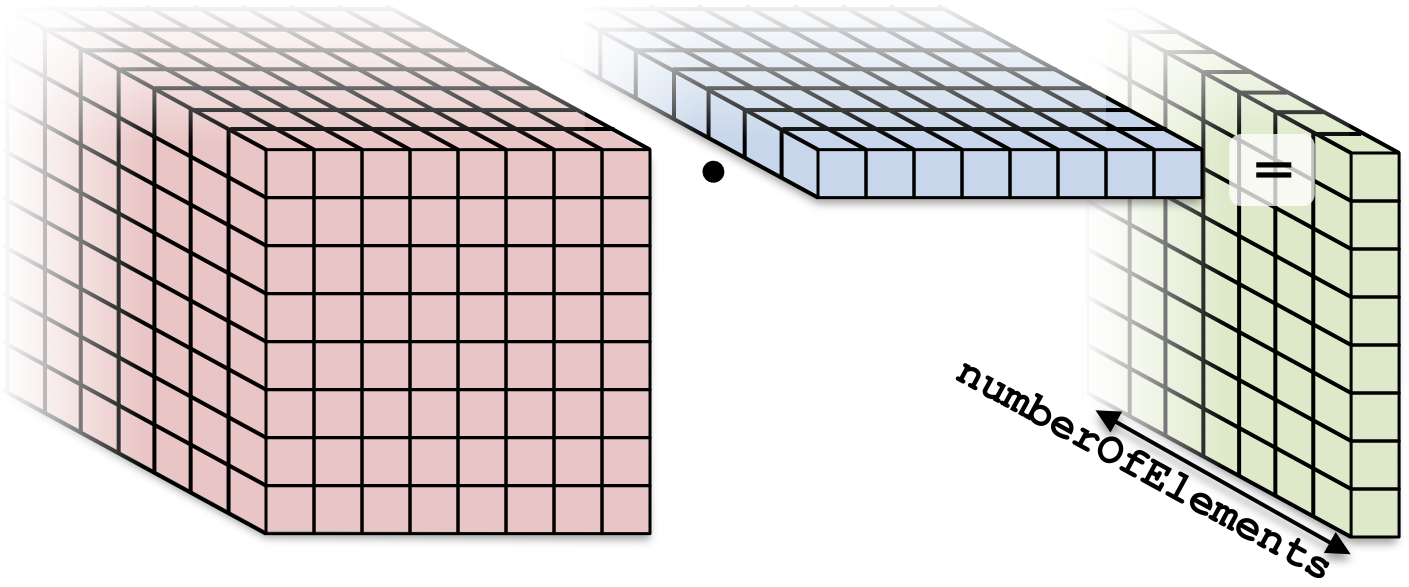
\includegraphics[width=0.75\textwidth]{figures/ContractDataFieldScalar}
  \end{center}

  \vspace{-10pt}

  \begin{code}[frame=single, keywords={}]
for (element = 0; element < numberOfElements; ++element) {
  for (qp = 0; qp < numberOfQPs; ++qp) {
    total = 0;
    for (i = 0; i < vectorSize; ++i) {
      total += @darkredA@darkred(element, qp, i) * @blueB@blue(element, i);
    }
    @darkgreenresult@darkgreen(element, qp) = total;
  }
}
  \end{code}

\end{frame}

%==========================================================================

\begin{frame}[fragile]{Example: contractDataFieldScalar (3)}

  \begin{columns}[t,onlytextwidth]
    \column{.55\textwidth}
      \begin{center}
        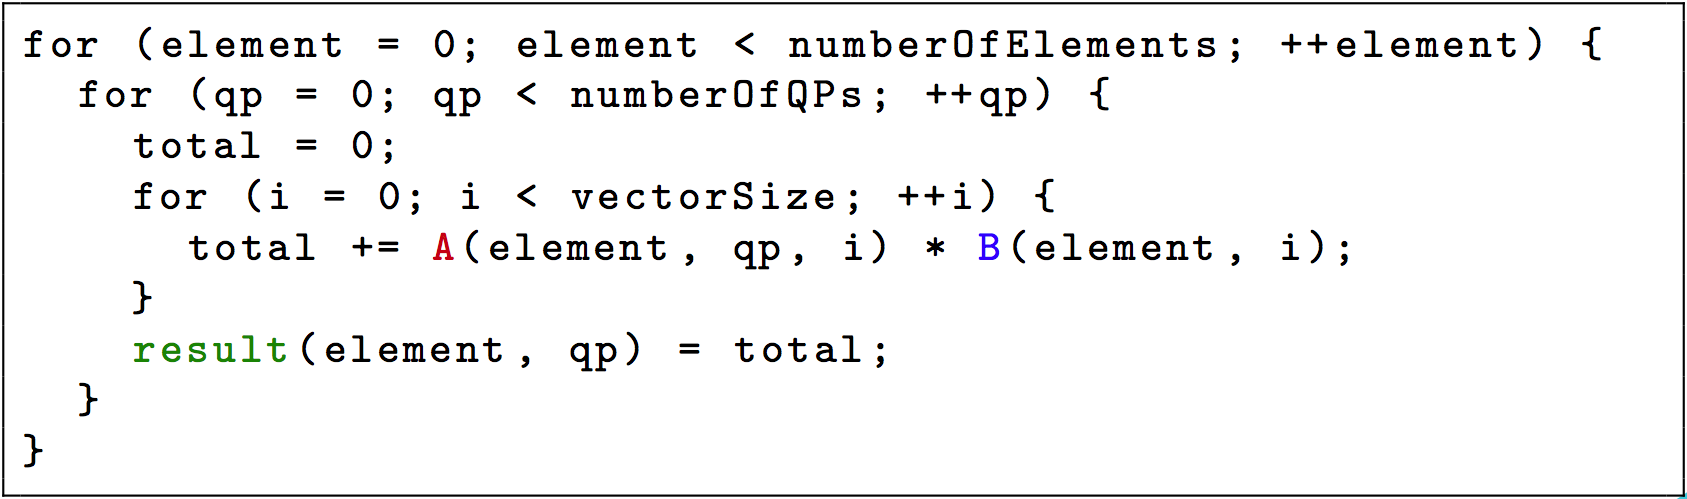
\includegraphics[width=1.00\textwidth]{figures/ContractDataFieldScalar_code}
      \end{center}
    \column{.45\textwidth}
      \begin{center}
        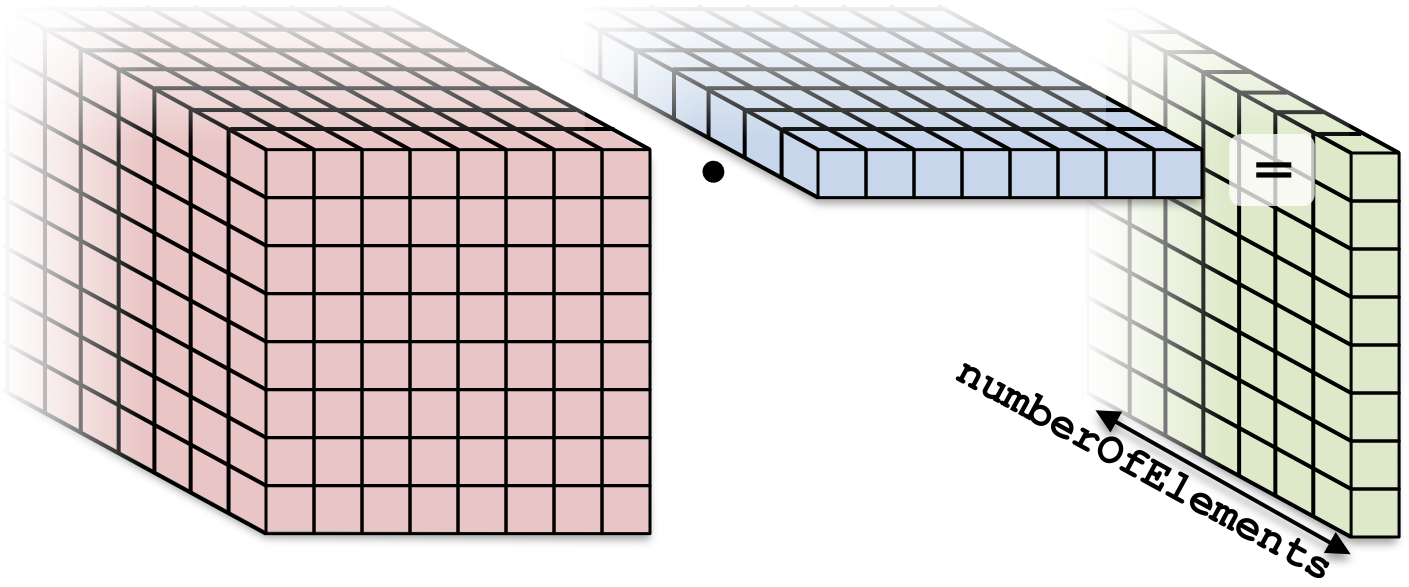
\includegraphics[width=1.00\textwidth]{figures/ContractDataFieldScalar}
      \end{center}
  \end{columns}

  \vspace{10pt}

  \ul{\textbf{Parallelization approaches:}}

  \begin{itemize}[<+->]
    \item{Each thread handles an \texttt{element}. \\
              \hspace{20pt} Threads: \texttt{numberOfElements}}
    \item \tikzmark{infrastructure}{Each thread handles a \texttt{qp}. \\
              \hspace{20pt} Threads: \texttt{numberOfElements * numberOfQPs}}
    \item{Each thread handles an \texttt{i}. \\
              \hspace{20pt} Threads: \texttt{numElements * numQPs * vectorSize}\\
              \hspace{20pt} \emph{Requires a} \texttt{parallel\_reduce}.}
  \end{itemize}

  \tikz[overlay,remember picture]{\draw<+->[draw=black,thick,fill opacity=0.2] ($(infrastructure)+(-0.5,0.4)$) rectangle ($(infrastructure)+(9,-0.6)$);}

\end{frame}

%==========================================================================

\begin{frame}[fragile]{Example: contractDataFieldScalar (4)}

  \begin{columns}[t,onlytextwidth]
    \column{.55\textwidth}
      \begin{center}
        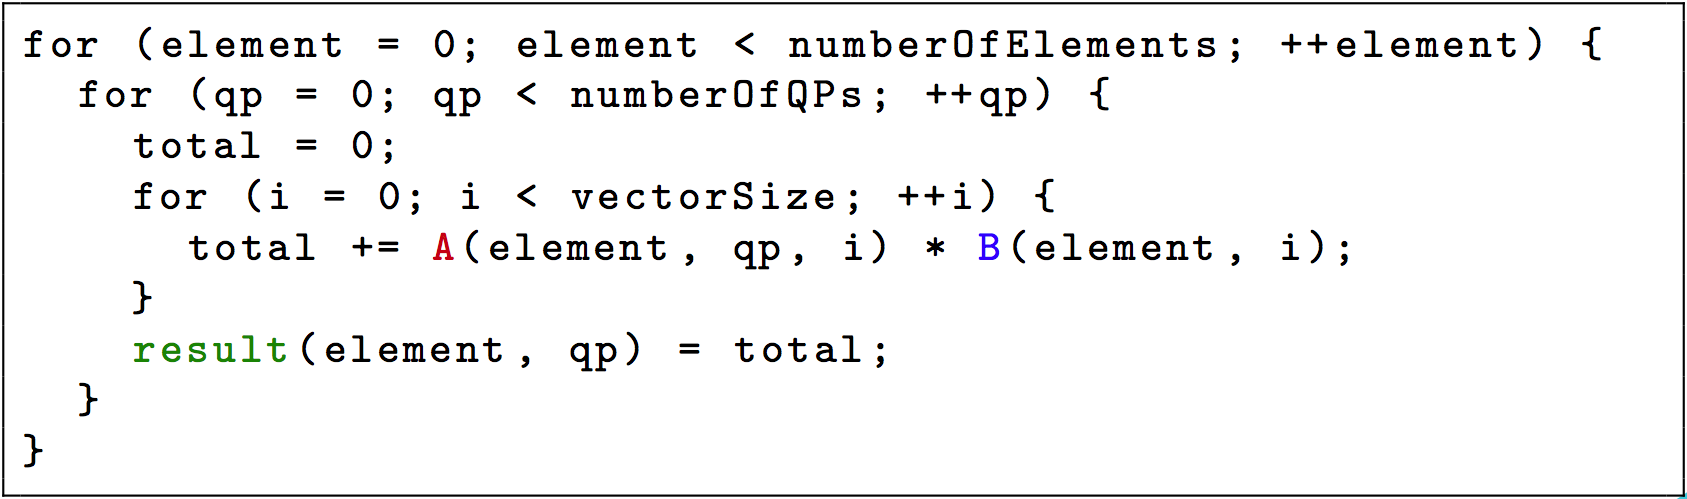
\includegraphics[width=1.00\textwidth]{figures/ContractDataFieldScalar_code}
      \end{center}
    \column{.45\textwidth}
      \begin{center}
        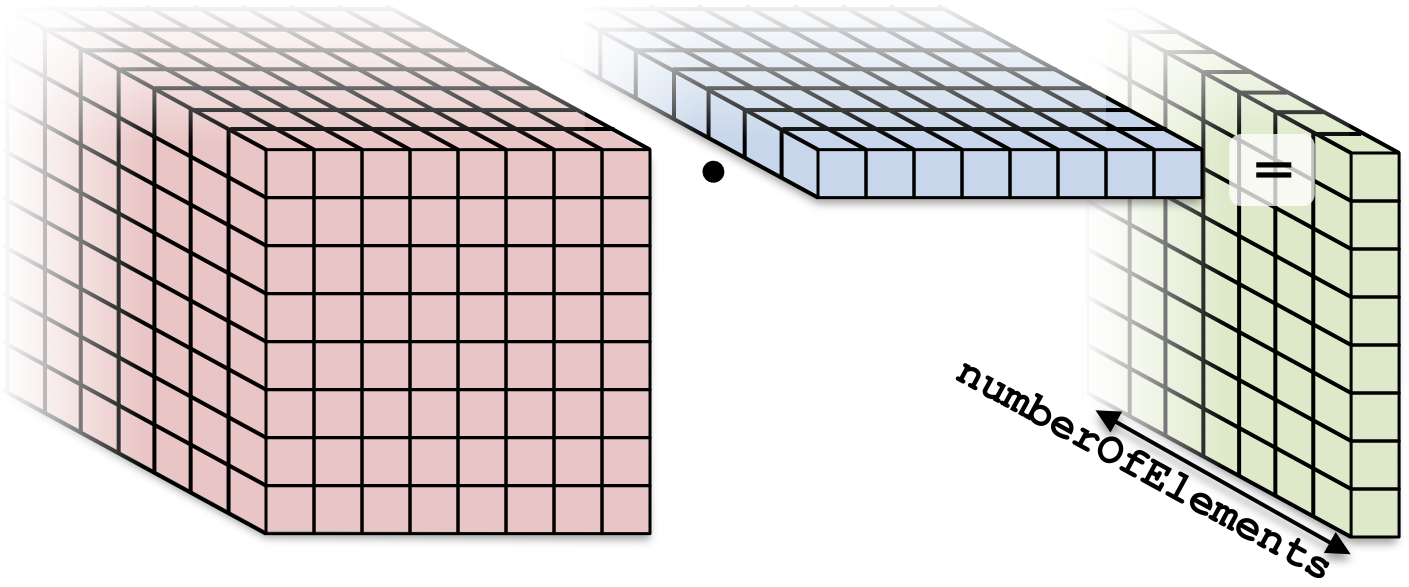
\includegraphics[width=1.00\textwidth]{figures/ContractDataFieldScalar}
      \end{center}
  \end{columns}

  \vspace{10pt}

  \ul{\textbf{Flat kernel:} Each thread handles a quadrature point}

  \begin{code}[frame=single, keywords={}]
parallel_for("L",MDRangePolicy<Rank<2>>({0,0},{numE,numQP}),
  KOKKOS_LAMBDA(int element, int qp) {
  @graydouble total = 0;
  for (int i = 0; i < vectorSize; ++i) {
    total += A(element, qp, i) * B(element, i);
  }
  result(element, qp) = total;@gray
}
  \end{code}

\end{frame}


\begin{frame}[fragile]{Example: contractDataFieldScalar (6)}

  \begin{columns}[t,onlytextwidth]
    \column{.55\textwidth}
      \begin{center}
        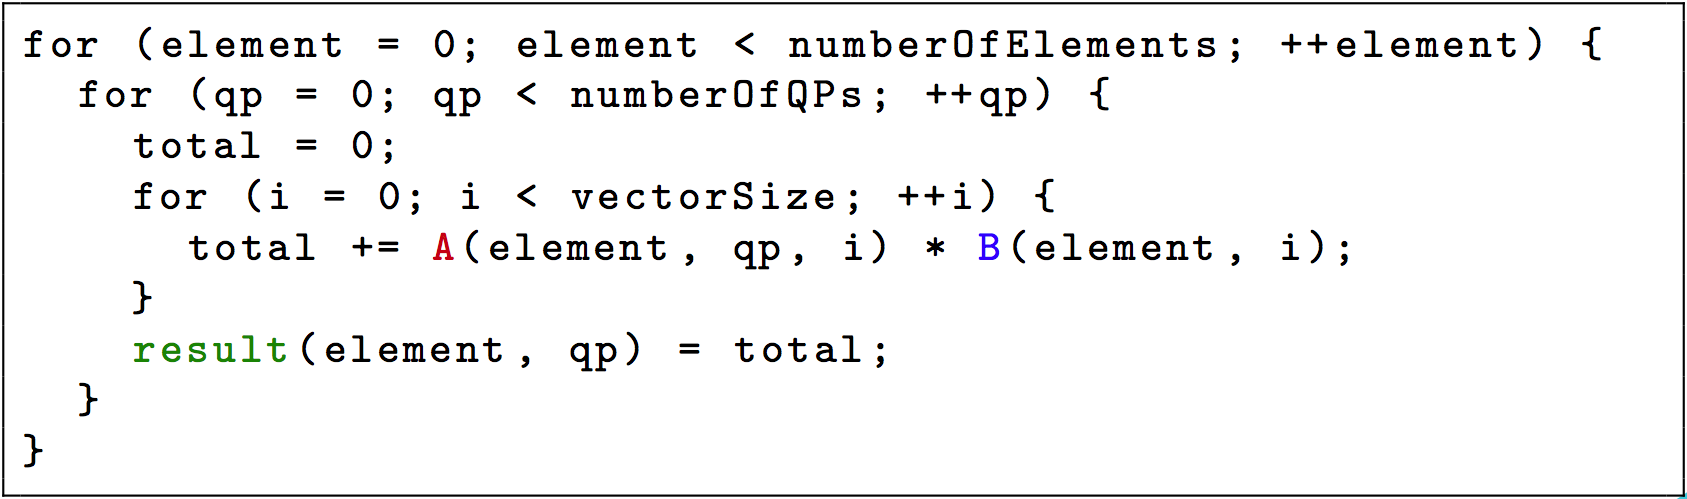
\includegraphics[width=1.00\textwidth]{figures/ContractDataFieldScalar_code}
      \end{center}
    \column{.45\textwidth}
      \begin{center}
        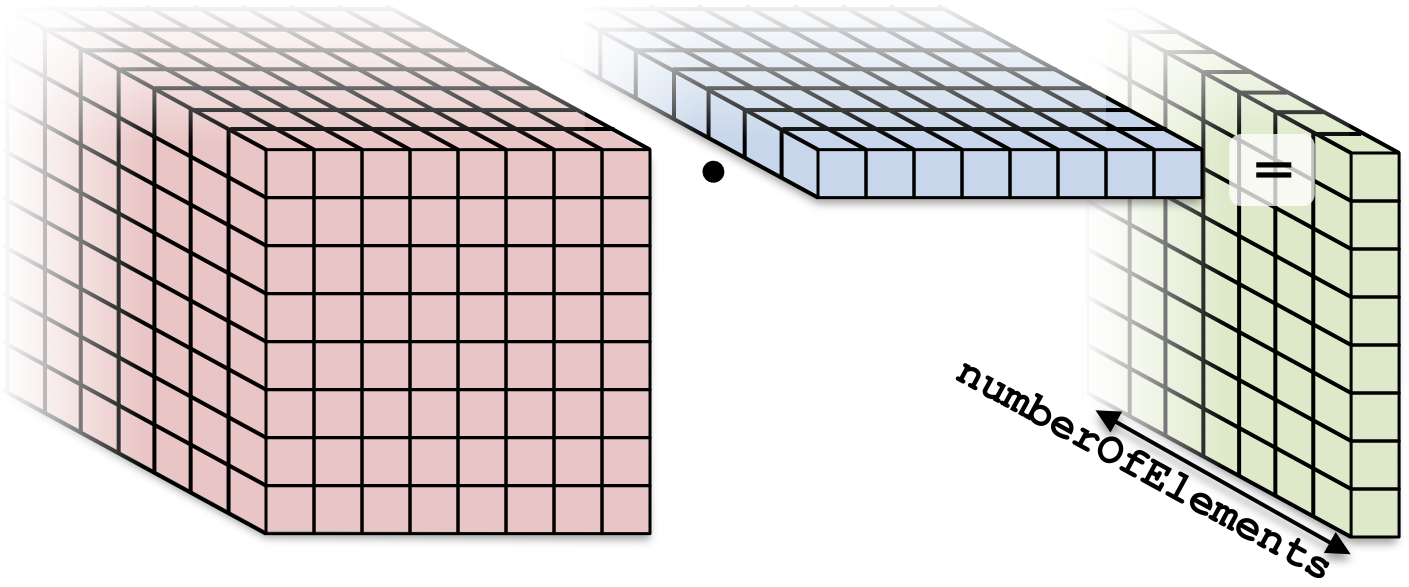
\includegraphics[width=1.00\textwidth]{figures/ContractDataFieldScalar}
      \end{center}
  \end{columns}

  \vspace{0pt}

  \ul{\textbf{Teams kernel:} Each team handles an element}

  \begin{code}[frame=single, keywords={}]
operator()(member_type teamMember) {
  int element = teamMember.league_rank();
  parallel_for(
    TeamThreadRange(teamMember, numberOfQPs),
    [=] (int qp) {
      @graydouble total = 0;
      for (int i = 0; i < vectorSize; ++i) {
        total += A(element, qp, i) * B(element, i);
      }
      result(element, qp) = total;@gray
    });
}
  \end{code}

  \begin{textblock*}{0.50\textwidth}(0.70\textwidth,0.865\textheight)
\only<2->{No real advantage (yet)}
  \end{textblock*}
\end{frame}

%==========================================================================

\begin{frame}[fragile]{Scratch memory (0)}

  Each team has access to a ``scratch pad''.

  \vspace{-10pt}

  \begin{center}
    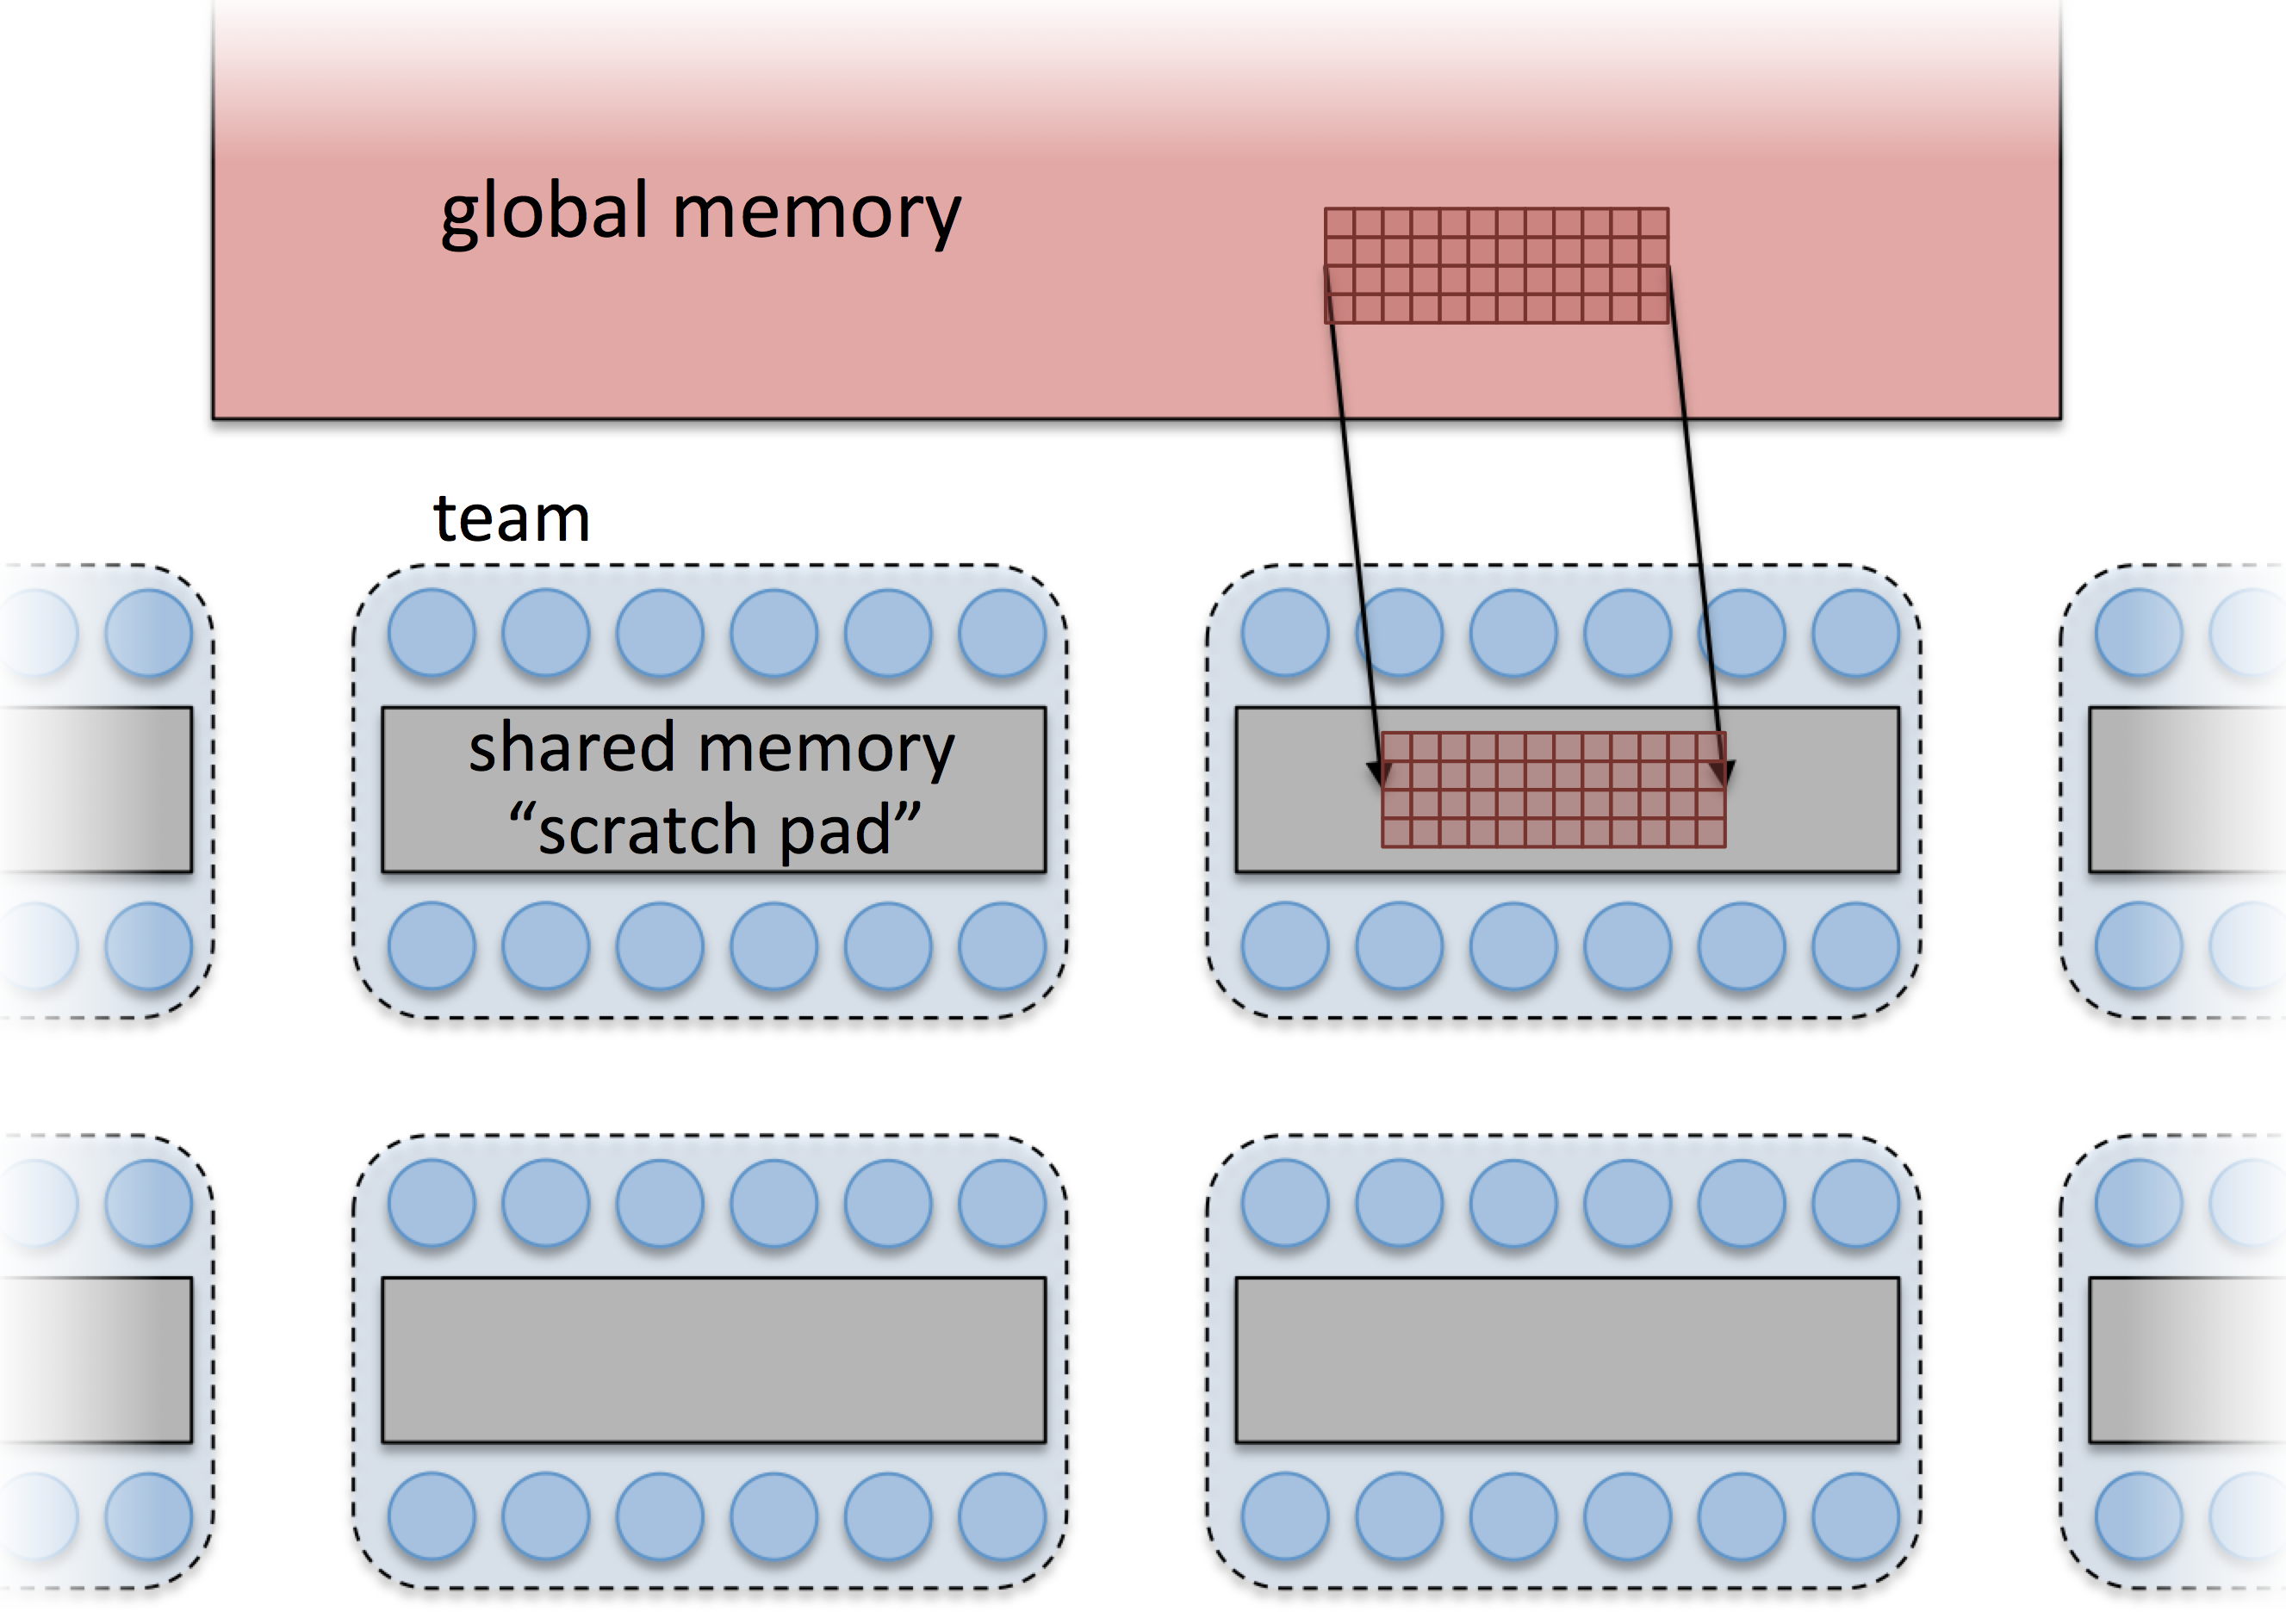
\includegraphics[width=0.90\textwidth]{figures/Hierarchical_sharedMemory}
  \end{center}

\end{frame}

%==========================================================================

\begin{frame}[fragile]{Scratch memory (1)}

  \textbf{Scratch memory (scratch pad) as manual cache:}

  \begin{itemize}
    \item{Accessing data in (level 0) scratch memory is (usually) \textbf{much faster} than global memory.}
    \item{\textbf{GPUs} have separate, dedicated, small, low-latency scratch memories (\emph{NOT subject to coalescing requirements}).}
    \item{\textbf{CPUs} don't have special hardware, but programming with scratch memory results in cache-aware memory access patterns.}
    \item{Roughly, it's like a \emph{user-managed} L1 cache.}
  \end{itemize}

  \pause

  \begin{block}{Important concept}
    When members of a team read the same data multiple times, it's better to load the data into scratch memory and read from there.
  \end{block}

\end{frame}

%==========================================================================

\begin{frame}[fragile]{Scratch memory (2)}

  \textbf{Scratch memory for temporary per work-item storage:}

  \begin{itemize}
    \item{Scenario: Algorithm requires temporary workspace of size W.}
    \item{\textbf{Without scratch memory:} pre-allocate space for N work-items of size N x W.}
    \item{\textbf{With scratch memory:} Kokkos pre-allocates space for each Team or Thread of size T x W.}
    \item{\texttt{PerThread} and \texttt{PerTeam} scratch can be used concurrently.}
    \item{Level 0 and Level 1 scratch memory can be used concurrently.}
  \end{itemize}

  \pause

  \begin{block}{Important concept}
    If an algorithm requires temporary workspace for each work-item, then use Kokkos' scratch memory.
  \end{block}

\end{frame}

%==========================================================================

\begin{frame}[fragile]{Scratch memory (3)}

  To use scratch memory, you need to:
  \begin{enumerate}
    \item{\textbf{Tell Kokkos how much} scratch memory you'll need.}
    \item{\textbf{Make} scratch memory \textbf{views} inside your kernels.}
  \end{enumerate}

  \pause
  \begin{code}
  TeamPolicy<ExecutionSpace> policy(numberOfTeams, teamSize);

  // Define a scratch memory view type
  using ScratchPadView =
      View<double*,@darkredExecutionSpace::scratch_memory_space@darkred>;
  // Compute how much scratch memory (in bytes) is needed
  size_t bytes = ScratchPadView::shmem_size(vectorSize);

  // Tell the policy how much scratch memory is needed
  int level = 0;
  parallel_for(policy.set_scratch_size(level, PerTeam(bytes)),
    KOKKOS_LAMBDA (const member_type& teamMember) {

      // Create a view from the pre-existing scratch memory
      ScratchPadView scratch(teamMember.@darkredteam_scratch(level)@darkred,
                             vectorSize);
  });
  \end{code}
\end{frame}

%==========================================================================

\begin{frame}[fragile]{Example: contractDataFieldScalar (7)}

  \ul{\textbf{Kernel outline for teams with scratch memory:}}

  \begin{code}[keywords={}]
@grayoperator()(member_type teamMember) {@gray
  ScratchPadView @bluescratch@blue(teamMember.team_scratch(0),
                         vectorSize);
  // TODO: load slice of B into scratch

  @grayparallel_for(
    TeamThreadRange(teamMember, numberOfQPs),
    [=] (int qp) {
      double total = 0;
      for (int i = 0; i < vectorSize; ++i) {@gray
        // total += A(element, qp, i) * B(element, i);
        total += A(element, qp, i) * @bluescratch@blue(i);
      @gray}
      result(element, qp) = total;
    });
}@gray
  \end{code}

  \begin{tikzpicture}[remember picture, overlay]
    \node [shift={(-5.6cm,0.85cm)}]  at (current page.south east)
      {%
      \begin{tikzpicture}[remember picture, overlay]
        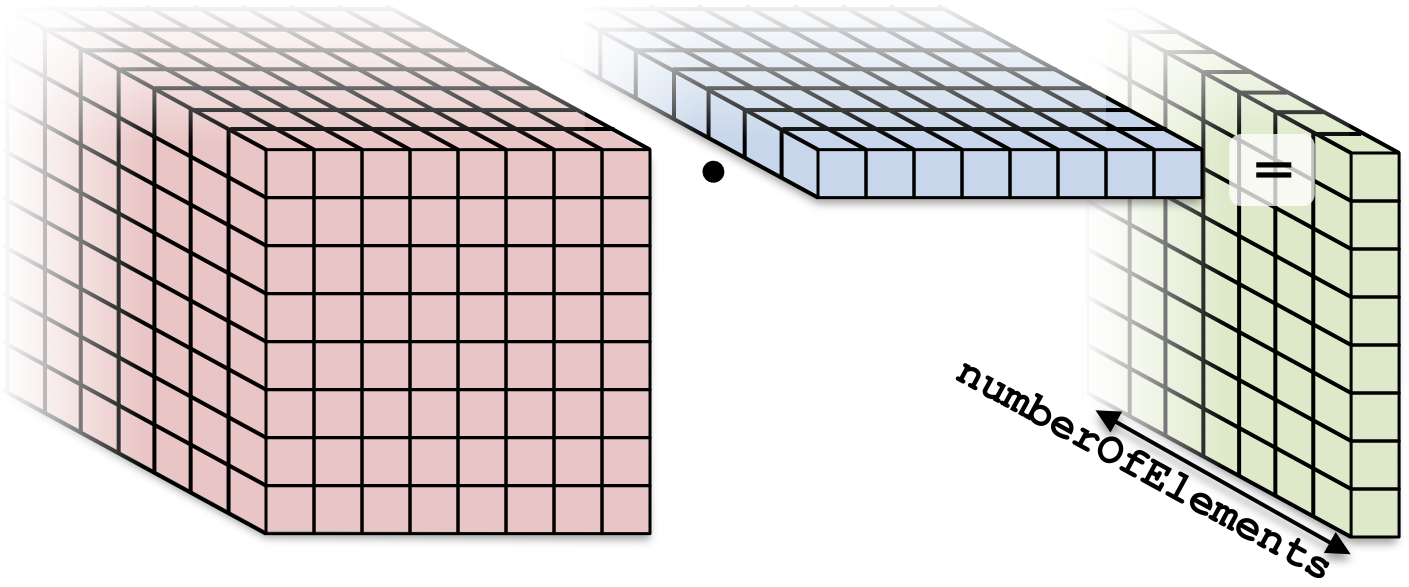
\includegraphics[width=0.45\textwidth]{figures/ContractDataFieldScalar}
      \end{tikzpicture}
      };
  \end{tikzpicture}

\end{frame}

%==========================================================================

\begin{frame}[fragile]{Example: contractDataFieldScalar (8)}

  \begin{tikzpicture}[remember picture, overlay]
    \node [shift={(-5.6cm,0.85cm)}]  at (current page.south east)
      {%
      \begin{tikzpicture}[remember picture, overlay]
        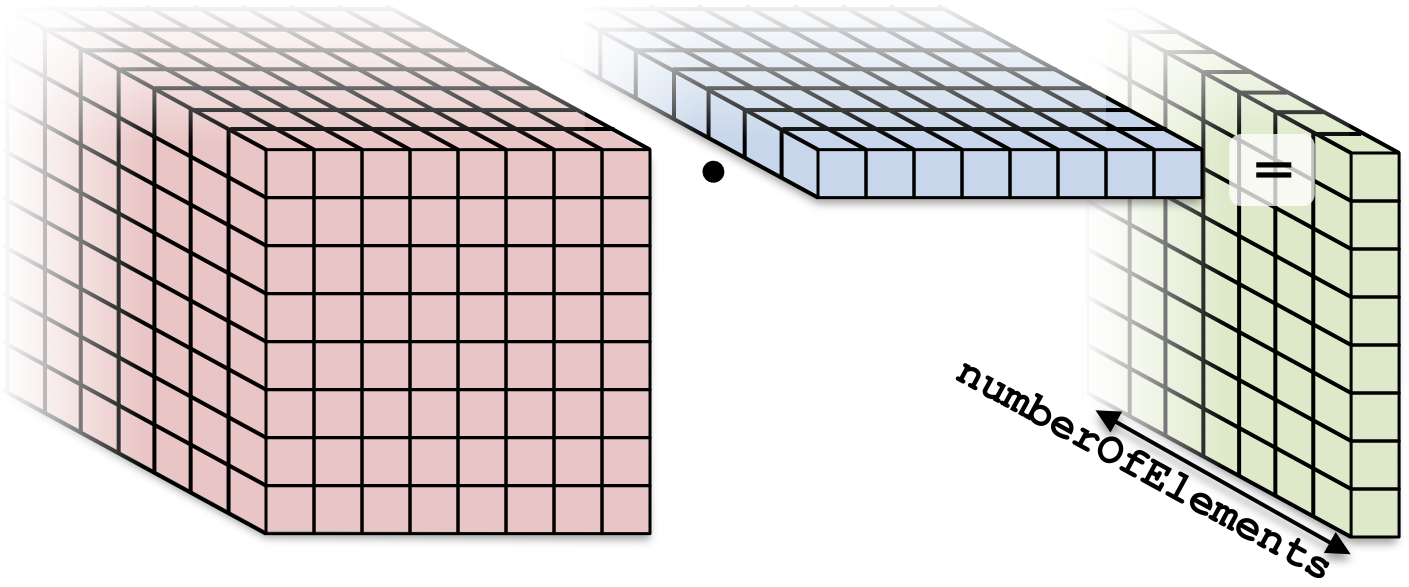
\includegraphics[width=0.45\textwidth]{figures/ContractDataFieldScalar}
      \end{tikzpicture}
      };
  \end{tikzpicture}

  \ul{\textbf{How to populate the scratch memory?}}

  \begin{itemize}
    \item<1->\only<1>{One thread loads it all?}\only<2->{\st{One thread loads it all?} \hspace{10pt} {\color{red}Serial}}

  \begin{code}[keywords={}]
if (teamMember.team_rank() == 0) {
  for (int i = 0; i < vectorSize; ++i) {
    @bluescratch@blue(i) = B(element, i);
  }
}
  \end{code}

    \item<2->\only<2>{Each thread loads one entry?}\only<3->{\st{Each thread loads one entry?} \hspace{10pt} {\color{red}\texttt{teamSize $\neq$ vectorSize}}}

  \only<1>{\hspace{0pt}}

  \onslide<2->

  \begin{code}[keywords={}]
@bluescratch@blue(team_rank) = B(element, team_rank);
  \end{code}

    \item<3->\tikzmark{left}\only<3-4>{\texttt{TeamVectorRange}}\tikzmark{right}

  \only<1-2>{\hspace{0pt}}

  \onslide<3->

  \begin{code}[keywords={}]
parallel_for(
  TeamVectorRange(teamMember, vectorSize),
  [=] (int i) {
    @bluescratch@blue(i) = B(element, i);
  });
  \end{code}

  \end{itemize}

  \only<4>{\DrawBoxWideBlack*[thick]}

  \vspace{50pt}

\end{frame}

%==========================================================================

\begin{frame}[fragile]{Example: contractDataFieldScalar (9)}

  \ul{\textbf{(incomplete) Kernel for teams with scratch memory:}}

  \begin{code}[keywords={}]
@grayoperator()(member_type teamMember) {@gray
  ScratchPadView @bluescratch@blue(...);

  @grayparallel_for(TeamVectorRange(teamMember, vectorSize),
    [=] (int i) {@gray
      @bluescratch@blue(i) = B(element, i);
    @gray});@gray
  // TODO: fix a problem at this location

  @grayparallel_for(TeamThreadRange(teamMember, numberOfQPs),
    [=] (int qp) {
      double total = 0;
      for (int i = 0; i < vectorSize; ++i) {@gray
        total += A(element, qp, i) * @bluescratch@blue(i);
      @gray}
      result(element, qp) = total;
    });
}@gray
  \end{code}

  \pause
  \vspace{-5pt}

  {\color{red}Problem}: threads may start to use {\color{blue}\texttt{scratch}} before all threads are done loading.

\end{frame}

%==========================================================================

\begin{frame}[fragile]{Example: contractDataFieldScalar (10)}

  \ul{\textbf{Kernel for teams with scratch memory:}}

  \begin{code}[keywords={}]
@grayoperator()(member_type teamMember) {@gray
  ScratchPadView @bluescratch@blue(...);

  @grayparallel_for(TeamVectorRange(teamMember, vectorSize),
    [=] (int i) {@gray
      @bluescratch@blue(i) = B(element, i);
    @gray});@gray
  @boldteamMember.team_barrier();@bold

  @grayparallel_for(TeamThreadRange(teamMember, numberOfQPs),
    [=] (int qp) {
      double total = 0;
      for (int i = 0; i < vectorSize; ++i) {@gray
        total += A(element, qp, i) * @bluescratch@blue(i);
      @gray}
      result(element, qp) = total;
    });
}@gray
  \end{code}

  \vspace{19pt}

  \begin{tikzpicture}[remember picture, overlay]
    \node [shift={(-5.6cm,0.85cm)}]  at (current page.south east)
      {%
      \begin{tikzpicture}[remember picture, overlay]
        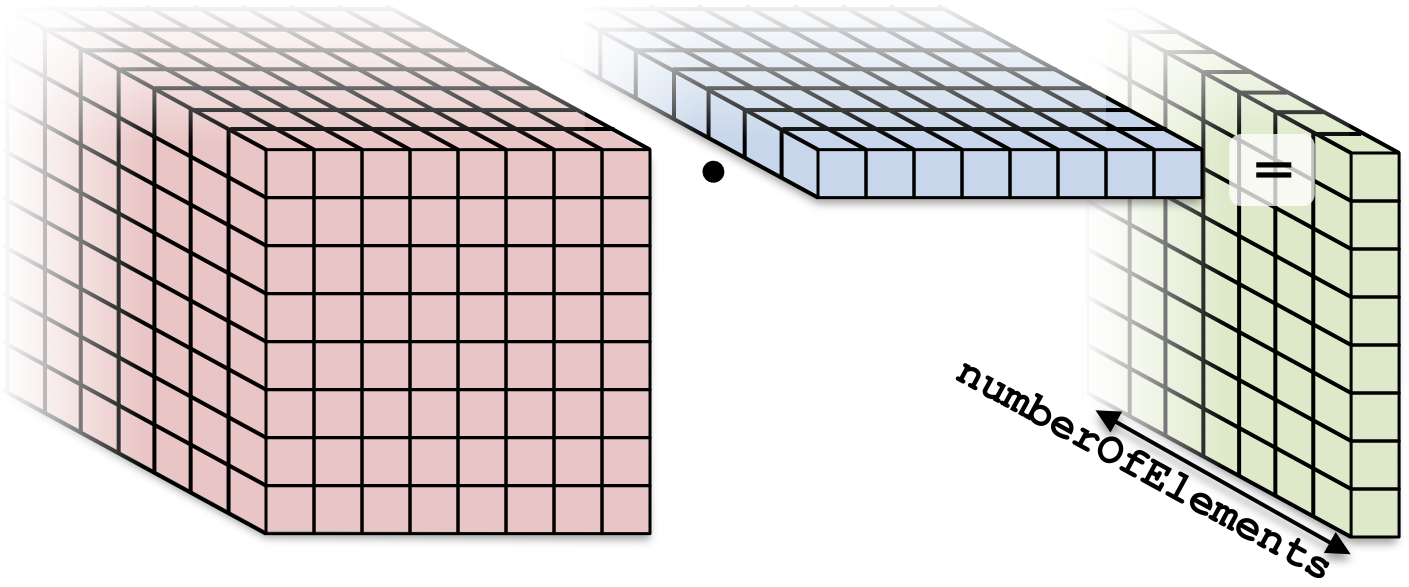
\includegraphics[width=0.50\textwidth]{figures/ContractDataFieldScalar}
      \end{tikzpicture}
      };
  \end{tikzpicture}

\end{frame}

%==========================================================================

\begin{frame}[fragile]{Exercise: Scratch Memory}
Use Scratch Memory to explicitly cache the x-vector for each element.

  \vspace{10pt}

  \textbf{Details}:
  \begin{small}
  \begin{itemize}
\item Location: \ExerciseDirectory{team\_scratch\_memory}
\item Create a scratch view
\item Fill the scratch view in parallel using a TeamVectorRange
\end{itemize}
  \end{small}

\ul{\textbf{Things to try:}}
  \begin{small}
  \begin{itemize}
  \item Vary problem size and number of rows (-S ...; -N ...)
  \item Compare behavior with Exercise 6
  \item Compare behavior of CPU vs GPU
  \end{itemize}
  \end{small}
\end{frame}

%==========================================================================

\begin{frame}[fragile]{Exercise: Scratch Memory}

  %\vspace{-10pt}

    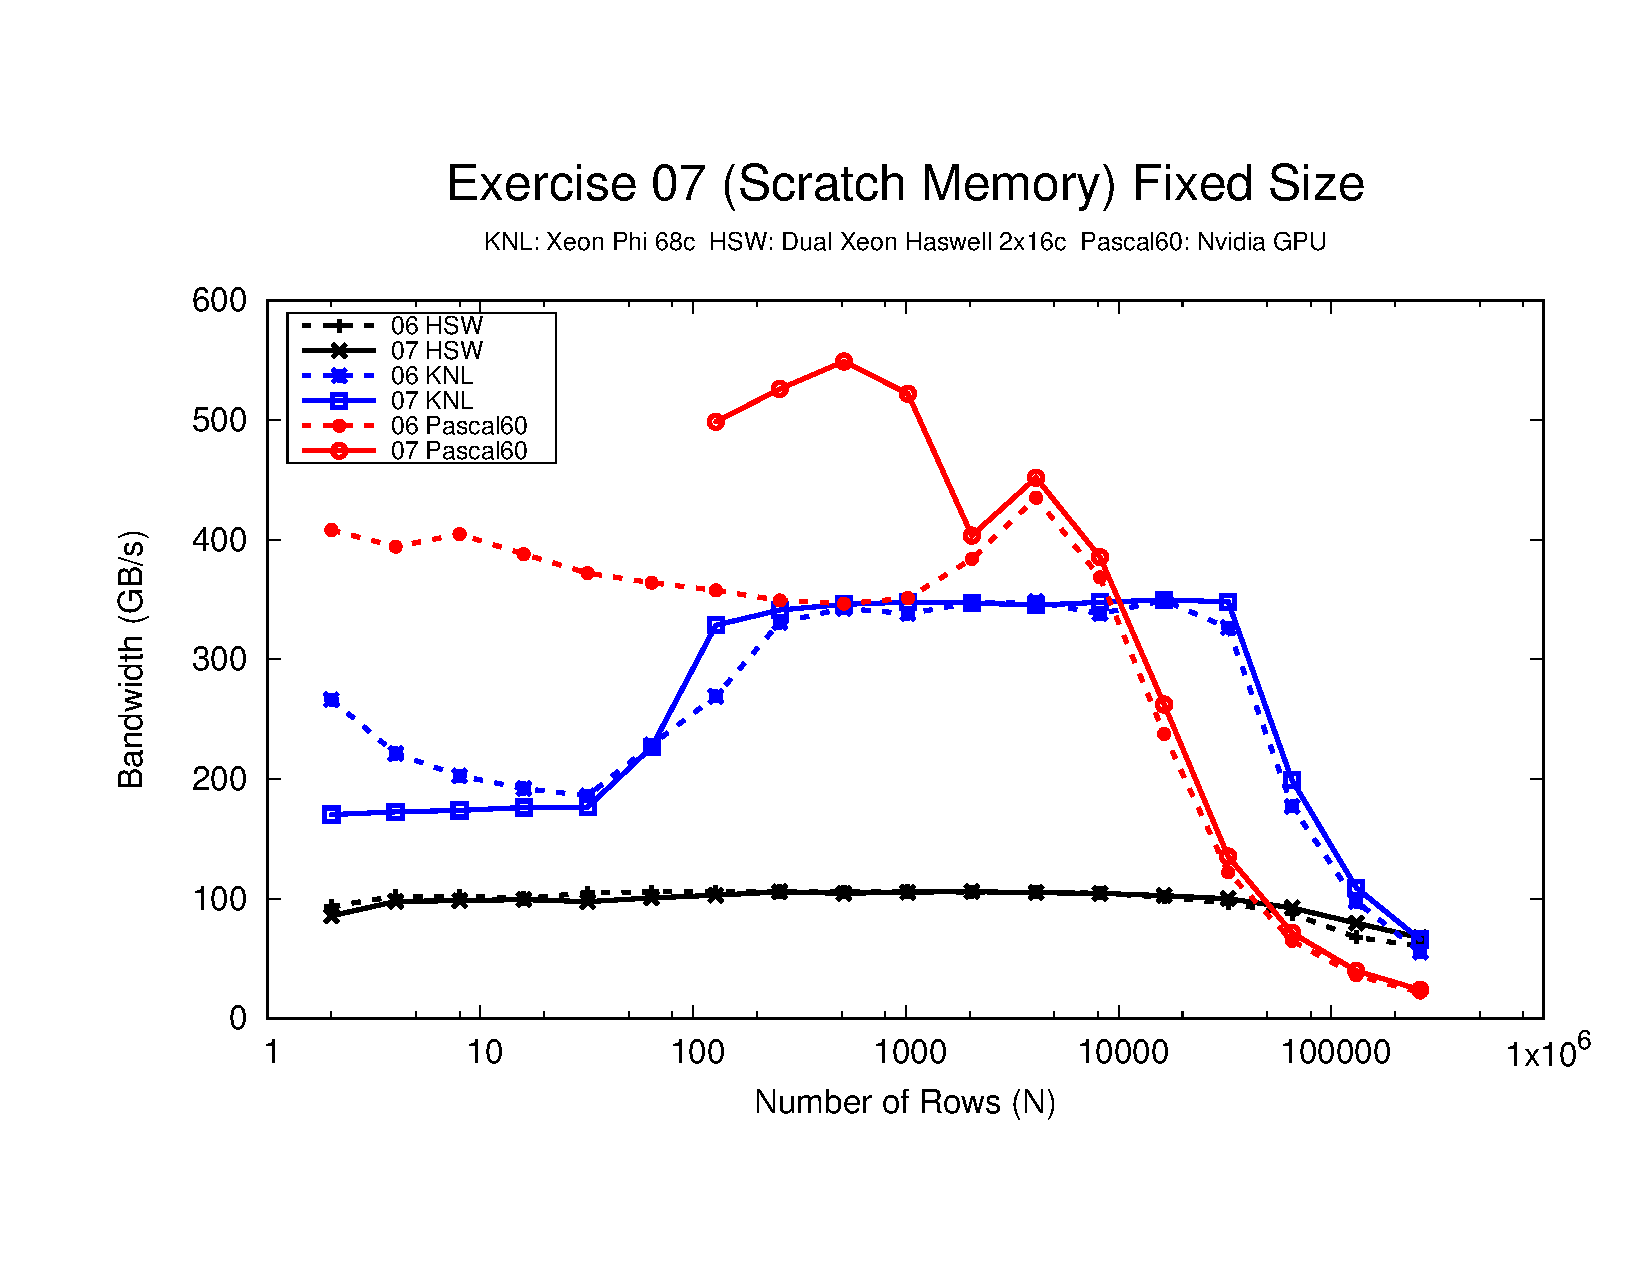
\includegraphics[viewport=1.25in 3.0in 10in 6in, width=0.95\textwidth]{figures/Exercise07-Performance.pdf}

  \vspace{-15pt}

\end{frame}

%==========================================================================

\begin{frame}[fragile]{Scratch Memory: API Details}
Allocating scratch in different levels:
  \begin{code}[keywords=level]
  int level = 1; // valid values 0,1
  policy.set_scratch_size(level,PerTeam(bytes));
  \end{code}

\pause

Using PerThread, PerTeam or both:
  \begin{code}[keywords={PerTeam,PerThread}]
  policy.set_scratch_size(level,PerTeam(bytes));
  policy.set_scratch_size(level,PerThread(bytes));
  policy.set_scratch_size(level,PerTeam(bytes1),
                                PerThread(bytes2));
  \end{code}

\pause

Using both levels of scratch:
  \begin{code}[keywords={PerTeam,PerThread}]
  policy.set_scratch_size(0,PerTeam(bytes0))
        .set_scratch_size(1,PerThread(bytes1));
  \end{code}

Note: \texttt{set\_scratch\_size()} returns a new policy instance, it doesn't modify the existing one.
\end{frame}

%==========================================================================

\begin{frame}{Section Summary}

  \begin{itemize}
    \item{\textbf{Scratch Memory} can be use with the \texttt{TeamPolicy} to provide thread or team \textbf{private} memory.}
    \item{Usecase: per work-item temporary storage or manual caching.}
    \item{Scratch memory exposes on-chip user managed caches (e.g. on NVIDIA GPUs)}
    \item{The size must be determined before launching a kernel.}
    \item{Two levels are available: large/slow and small/fast.}
  \end{itemize}

\end{frame}

%==========================================================================

\begin{frame}[fragile]{}

  {\Huge{Unique Token}}

  \vspace{20pt}

  \textbf{Learning objectives:}
  \begin{itemize}
    \item {Understand concept of unique tokens and thread-safe resource access. }
    \item {Learn how to acquire per-team unique ids.}
    \item {Understand the difference between \textbf{Global} and \textbf{Instance} scope.}
  \end{itemize}

  \vspace{-20pt}

\end{frame}

%==========================================================================

\begin{frame}[fragile]{Unique Tokens - Motivation}
\textbf{Why do we need a unique token concept?}
\begin{itemize}
\item{Within Functor operator / Lambda there is no portable way to identify the active execution resource (thread id)}
\item{Some algorithms make efficient use of shared resources by dividing based on execution resource (thread id)}
\item{Thread Id is not consistent or portable across all execution environments}
\item{Unique Token provides consistent identifier for resource allocations and work division}
\end{itemize}

\end{frame}

%==========================================================================

\begin{frame}[fragile]{Unique Tokens - Motivation}
\textbf{Original Example: Random Number Generator Pool}

\begin{code}
int N = 10000000
int K = ...;
RandomGenPool pool(K,seed);
parallel_for("Loop", N, KOKKOS_LAMBDA(int i) {
  int gen_id = ...
  auto gen = pool[gen_id];
});
\end{code}

\vspace{5pt}
\textbf{How many generators do we need (\texttt{K})?}

\pause
\vspace{5pt}
\textbf{How to get a unique one in the loop (\texttt{gen\_id})?}

\pause
\vspace{5pt}
In OpenMP we could use the \textbf{thread-id} but what in CUDA?

\end{frame}

%==========================================================================

\begin{frame}[fragile]{Unique Tokens - Motivation}
\vspace{-10pt}
\textbf{Motivating Example}

\vspace{5pt}
\textbf{OpenMP}
    \begin{code}[frame=single, keywords={}]
int K = omp_get_max_threads();
Kokkos::parallel_for("L", N, KOKKOS_LAMBDA(int i) {
  int tid = omp_get_thread_num();
});
    \end{code}

\vspace{5pt}
\textbf{CUDA}
    \begin{code}[frame=single, keywords={}]
int K = N; // ??
Kokkos::parallel_for("L", N, KOKKOS_LAMBDA(int i) {
  int tid = threadIdx.x + blockDim.x * blockIdx.x; //i??
});
    \end{code}

\pause
  \textbf{{\color{red}Problem}}: In \textbf{CUDA} there is no way to get \textbf{hardware thread-id}.

  \vspace{5pt}
  \pause

  \textbf{Solution:} We need a thread-safe and portable way to obtain unique identifier that is per-thread specific.

  \vspace{5pt}

  \hspace{20pt}{\Large $\Rightarrow$ \textbf{UniqueToken}}

  \vspace{-5pt}

\end{frame}

%==========================================================================

\begin{frame}[fragile]{Unique Token}

\textbf{UniqueToken is a pool of IDs}

\begin{itemize}
\item User acquires an ID and releases it again.
\end{itemize}

   \begin{code}[frame=single, keywords={UniqueToken,size,acquire,release}]
    UniqueToken<ExecutionSpace> token;
    int number_of_uniqe_ids = token.size();
    RandomGenPool pool(number_of_unique_ids,seed);
    parallel_for("L", N, KOKKOS_LAMBDA(int i) {
      int id = token.acquire();
      RandomGen gen = pool(id);
      ...
      token.release(id);
    });
   \end{code}

\pause
\begin{itemize}
\item Do not acquire more than one token in an iteration.
\item You must release the token again.
\item By default the range of ids is 0 to \texttt{ExecSpace().concurrency()}.
\end{itemize}

\end{frame}

%==========================================================================

\begin{frame}[fragile]{Unique Token - Global vs. Instance Scope}

\textbf{Sometimes you need a Global UniqueToken}
\begin{itemize}
\item Submitting concurrent kernels to CUDA streams (Module 5)
\item Shared resource in a multi-threaded environment like Legion
\end{itemize}

\vspace{-5pt}
\pause
\begin{block}{UniqueToken is Scoped}
UniqueToken has a Scope template parameter which by default is 'Instance' but can be 'Global'.
\end{block}

\pause
   \begin{code}[frame=single, keywords={UniqueTokenScope,Global,stream1,stream2}]
void foo() {
  UniqueToken<ExecSpace,UniqueTokenScope::Global> token_foo;
  parallel_for("L", RangePolicy<ExecSpace>(stream1,0,N)
    , functor_a(token_foo));
}
void bar() {
  UniqueToken<ExecSpace,UniqueTokenScope::Global> token_bar;
  parallel_for("L", RangePolicy<ExecSpace>(stream2,0,N)
    , functor_b(token_bar));
}
   \end{code}

\pause
\texttt{token\_foo} and \texttt{token\_bar} will provide non-conflicting ids.
\end{frame}
%==========================================================================

\begin{frame}[fragile]{Unique Token - Per Team}

  \textbf{UniqueToken can also be used for Per-Team resources}

\vspace{5pt}
  There are less teams active than threads. How to get an ID?

\vspace{5pt}
\pause
\begin{block}{Sized UniqueToken}
{UniqueToken supports custom ranges of ids via constructing sized tokens.}
\end{block}

\pause
\textbf{Acquiring a per-team unique id requires three steps:}
\begin{itemize}
  \item Compute the range via \texttt{concurrency} and \texttt{team\_size}.
  \item Create a sized \texttt{UniqueToken}.
  \begin{itemize}
    \item For performance reason make it a bit larger than necessary.
  \end{itemize}
  \item Acquire and broadcast a token in a \texttt{single} pattern.
\end{itemize}
\end{frame}

\begin{frame}[fragile]{Unique Token - Per Team}

   \begin{code}[frame=single, keywords={team_size,concurrency,token,single,PerTeam}]
// Figure out the team size
int team_size = ...;
// How many teams are actually in-flight
int num_active_teams = ExecSpace().concurrency()/team_size;
// Create the token
UniqueToken<ExecSpace> token(num_active_teams * 1.2);

parallel_for("L", TeamPolicy<ExecSpace>(N,team_size),
  KOKKOS_LAMBDA(const team_t& team) {
    int id;
    // Acquire an id and broadcast it with a single thread
    single(PerTeam(team),[&](int &lid) {
      lid = token.acquire();
    },id);
    ...
    // Release the id again (likely you want a barrier first!)
    single(PerTeam(team),[&]() {
      token.release(id);
    });
   \end{code}


\end{frame}

%==========================================================================


\begin{frame}[fragile]{Exercise UniqueToken}

  \begin{small}
  \begin{itemize}
  \item Location: \ExerciseDirectory{unique\_token/Begin}
  \item Assignment: Convert scatter\_add\_loop to use \texttt{UniqueToken}, removing \#ifdef's
  \item Compile and run on both CPU and GPU
  \end{itemize}
  \end{small}

\begin{code}
make -j KOKKOS_DEVICES=OpenMP  # CPU-only using OpenMP
make -j KOKKOS_DEVICES=Cuda    # GPU - note UVM in Makefile 
# Run exercise
./uniquetoken.host
./uniquetoken.cuda
# Note the warnings, set appropriate environment variables
\end{code}

  \begin{scriptsize}
  \begin{itemize}
  \item Compare performance on CPU of the three variants
  \item Compare performance on GPU of the two variants
  \item Vary problem size: first and second optional argument
  \end{itemize}
  \end{scriptsize}

\end{frame}

%==========================================================================

\begin{frame}{Section Summary}

  \begin{itemize}
    \item{\textbf{UniqueToken} provides a thread safe portable way to divide thread or team specific resources}
    \item{\textbf{UniqueToken} can be sized, such that it returns only ids within a specific range.}
    \item{A \textbf{Global} scope UniqueToken can be acquired, allowing safe ids accross disjoint concurrent code sections.}
  \end{itemize}

\end{frame}



\begin{frame}[fragile]{Module 4: Summary}
	\textbf{Hierarchal Parallelism}
  \begin{itemize}
    \item{\textbf{Hierarchical work} can be parallelized via hierarchical parallelism.}
    \item{Hierarchical parallelism is leveraged using \textbf{thread teams} launched with a \texttt{TeamPolicy}.}
    \item{Team ``worksets'' are processed by a team in nested \texttt{parallel\_for} (or \texttt{reduce} or \texttt{scan}) calls with a \texttt{TeamThreadRange} and \texttt{ThreadVectorRange} policy.}
    \item{Execution can be restricted to a subset of the team with the \texttt{single} pattern using either a \texttt{PerTeam} or \texttt{PerThread} policy.}
    \item{Teams can be used to \textbf{reduce contention} for global resources even in ``flat'' algorithms.}
  \end{itemize}


  
\end{frame}

\begin{frame}[fragile]{Module 4: Summary}
   \textbf{Scratch Space}
\begin{itemize}
    \item{\textbf{Scratch Memory} can be use with the \texttt{TeamPolicy} to provide thread or team \textbf{private} memory.}
    \item{Usecase: per work-item temporary storage or manual caching.}
    \item{Scratch memory exposes on-chip user managed caches (e.g. on NVIDIA GPUs)}
    \item{The size must be determined before launching a kernel.}
    \item{Two levels are available: large/slow and small/fast.}
  \end{itemize}
  \textbf{Unique Token}
  \begin{itemize}
    \item{\textbf{UniqueToken} give a thread safe portable way to divide thread specific resources}
    \item{\textbf{UniqueToken} can be sized to restrict ids to a range.}
    \item{A \textbf{Global} UniqueToken is available.}
  \end{itemize}

\end{frame}

\begin{frame}{Module 5: Outlook (08/14)}
    \vspace{-3pt}
	\textbf{Task Parallelism:}
	\begin{itemize}
        \item {Basic interface for fine-grained tasking in Kokkos}
        \item {How to express dynamic dependency structures in Kokkos}
	\end{itemize}
	
	\vspace{5pt}
	\textbf{Streams: Concurrent Execution Spaces}
	\begin{itemize}
		\item {How to use Streams within Kokkos Execution spaces}
	\end{itemize}

	\vspace{5pt}
	\textbf{SIMD: Portable vector intrinsic types}
	\begin{itemize}
		\item {How to use SIMD types to improve vectorization}
		\item {Alternative to ThreadVector loops and outer loop vectorization}
	\end{itemize}

	\vspace{5pt}
    \textbf{Slack channel:} {\scriptsize \url{https://kokkosteam.slack.com/}}
	
	\vspace{5pt}
	\textbf{Recordings/Slides:} {\scriptsize \url{https://kokkos.org/kokkos-core-wiki/videolectures.html}}

\end{frame}

\end{document}

